% lecture11.tex -- GENERATED by build_L11.py from L11_numbers.json; do not edit by hand.
\documentclass[10pt,aspectratio=169,t]{beamer}
% =============================================================================
% nn_preamble.tex -- shared Beamer preamble of Neural Networks and Deep Learning (NN)
% Used by every lecture: lectures/Lk/lecturek.tex does
%   \documentclass[10pt,aspectratio=169,t]{beamer}
%   % =============================================================================
% nn_preamble.tex -- shared Beamer preamble of Neural Networks and Deep Learning (NN)
% Used by every lecture: lectures/Lk/lecturek.tex does
%   \documentclass[10pt,aspectratio=169,t]{beamer}
%   % =============================================================================
% nn_preamble.tex -- shared Beamer preamble of Neural Networks and Deep Learning (NN)
% Used by every lecture: lectures/Lk/lecturek.tex does
%   \documentclass[10pt,aspectratio=169,t]{beamer}
%   \input{../common/nn_preamble}
%   \nnlecture{k}{Lecture title}
% Logos live in lectures/common/logos/, charts in lectures/Lk/charts/.
% Do NOT add \hfuzz / \vfuzz / \hbadness here: overfull boxes must be fixed, not hidden.
% =============================================================================

\usetheme{default}
\setbeamersize{text margin left=7mm, text margin right=7mm}

% ---------------------------------------------------------------- packages
\usepackage[utf8]{inputenc}
\usepackage[T1]{fontenc}
\usepackage{lmodern}
\usepackage{amsmath, amssymb}
\usepackage{mathtools}
\usepackage{bm}
\usepackage{tikz}
\usetikzlibrary{arrows.meta, positioning, calc, shapes.misc}
\usepackage{booktabs}
\usepackage{array}
\usepackage{graphicx}
\usepackage{colortbl}
\usepackage{xcolor}
\usepackage{multicol}
\hypersetup{colorlinks=true, linkcolor=MainBlue, urlcolor=MainBlue, citecolor=MainBlue}
\graphicspath{{../common/logos/}}   % charts are included with their language folder: charts/en/, charts/ro/

% ---------------------------------------------------------------- colours
\definecolor{MainBlue}{RGB}{26, 58, 110}
\definecolor{IDAred}{RGB}{205, 0, 0}
\definecolor{DarkGray}{RGB}{51, 51, 51}
\definecolor{FooterGray}{RGB}{100, 100, 100}
\definecolor{BlockGray}{RGB}{236, 238, 242}
\definecolor{KeynoteGray}{RGB}{218, 218, 218}
\definecolor{Crimson}{RGB}{190, 40, 50}
\definecolor{Forest}{RGB}{30, 110, 50}
\definecolor{Bitter}{RGB}{214, 150, 20}
% chart palette (same hex values and order as lectures/common/nn_plot.py SERIES)
\definecolor{Ser1}{HTML}{2A78D6}
\definecolor{Ser2}{HTML}{EB6834}
\definecolor{Ser3}{HTML}{1BAF7A}
\definecolor{Ser4}{HTML}{EDA100}
\definecolor{Ser5}{HTML}{E87BA4}
\definecolor{Ser6}{HTML}{008300}
\definecolor{Ser7}{HTML}{6250D6}
\definecolor{Ser8}{HTML}{E34948}

\setbeamertemplate{background}{%
  \begin{tikzpicture}[remember picture, overlay]
    \shade[shading=axis, shading angle=315, top color=white, bottom color=KeynoteGray]
      (current page.south west) rectangle (current page.north east);
  \end{tikzpicture}}
\setbeamercolor{background canvas}{bg=}
\setbeamercolor{structure}{fg=MainBlue}
\setbeamercolor{normal text}{fg=DarkGray}
\setbeamercolor{title}{fg=IDAred}
\setbeamercolor{frametitle}{fg=IDAred, bg=}
\setbeamercolor{block title}{bg=MainBlue, fg=white}
\setbeamercolor{block body}{bg=BlockGray, fg=DarkGray}
\setbeamercolor{block title alerted}{bg=Crimson, fg=white}
\setbeamercolor{block body alerted}{bg=Crimson!7, fg=DarkGray}
\setbeamercolor{block title example}{bg=Forest, fg=white}
\setbeamercolor{block body example}{bg=Forest!7, fg=DarkGray}
\setbeamercolor{item}{fg=MainBlue}
\setbeamerfont{frametitle}{size=\large, series=\bfseries}
\setbeamerfont{block title}{size=\small, series=\bfseries}
\setbeamertemplate{blocks}[rounded][shadow=false]
\setbeamertemplate{itemize item}{\color{MainBlue}$\boxdot$}
\setbeamertemplate{itemize subitem}{\color{MainBlue}\scriptsize$\blacktriangleright$}
% compact two-level lists: level 1 = main point, level 2 = details (no text outside bullets)
\setbeamerfont{itemize/enumerate subbody}{size=\footnotesize}
\setlength{\leftmargini}{1.1em}
\setlength{\leftmarginii}{1.1em}
\setbeamertemplate{itemize/enumerate body begin}{\setlength{\topsep}{0pt}\setlength{\partopsep}{0pt}\setlength{\parskip}{0pt}}
\setbeamertemplate{itemize/enumerate subbody begin}{\setlength{\topsep}{0pt}\setlength{\partopsep}{0pt}\setlength{\itemsep}{0pt}\vspace{-0.4ex}}

\setbeamertemplate{enumerate item}{\color{MainBlue}\insertenumlabel.}
\setlength{\leftmargini}{1.3em}
\setlength{\leftmarginii}{1.2em}
\setbeamertemplate{navigation symbols}{}
\setbeamertemplate{section in toc}{\color{MainBlue}$\blacktriangleright$~\inserttocsection}
\setbeamertemplate{caption}{\raggedright\insertcaption\par}
% frame subtitle = precise citation line under the claim title (Weron style)
\setbeamerfont{framesubtitle}{size=\footnotesize}
\setbeamercolor{framesubtitle}{fg=FooterGray}
% outline that reappears at every section with the current section highlighted
\setbeamertemplate{section in toc shaded}[default][35]
\setbeamertemplate{subsection in toc shaded}[default][35]
\setbeamertemplate{subsection in toc}{\leavevmode\leftskip=2.2em\color{DarkGray}\small\inserttocsubsection\par}
\AtBeginSection[]{{\begin{frame}{\txtoutline}\vspace{2mm}\small
  \tableofcontents[currentsection,hideothersubsections]\end{frame}}}

% ---------------------------------------------------------------- head and foot
\setbeamertemplate{headline}{%
  \vskip10pt%
  \hbox to \paperwidth{\hskip0.5cm%
    {\small\color{FooterGray}\renewcommand{\hyperlink}[2]{##2}\insertsectionhead}%
    \hfill\textcolor{FooterGray}{\small\insertframenumber}\hskip0.5cm}%
  \vskip4pt{\color{FooterGray}\hrule height 0.4pt}}
% footer as in the other courses (MFM, SFM): course name on the left, small sparkline on the right
\setbeamertemplate{footline}{%
  {\color{FooterGray}\hrule height 0.4pt}\vskip4pt%
  \hbox to \paperwidth{\hskip0.5cm%
    \textcolor{FooterGray}{\small\txtcourse}%
    \hfill\raisebox{-0.1em}{\begin{tikzpicture}[x=0.08em, y=0.08em, line width=0.4pt]
      \draw[FooterGray] (0,3) -- (1,4) -- (2,3.5) -- (3,5) -- (4,4) -- (5,6) -- (6,5.5) -- (7,4) -- (8,5) -- (9,7) -- (10,6) -- (11,5) -- (12,6.5) -- (13,8) -- (14,7) -- (15,6) -- (16,7.5) -- (17,9) -- (18,8) -- (19,7) -- (20,8.5) -- (21,10) -- (22,9) -- (23,8) -- (24,9.5);
    \end{tikzpicture}}\hskip0.5cm}%
  \vskip6pt}

% ---------------------------------------------------------------- title page
\defbeamertemplate*{title page}{nn}[1][]{%
  \vspace{0.15cm}
  \begin{center}
    \href{https://www.ase.ro}{
\includegraphics[height=0.9cm]{ase_logo.png}}\hspace{0.3cm}%
    \href{https://ipe.ro/new}{
\includegraphics[height=0.9cm]{acad_logo.png}}\hspace{0.3cm}%
    \href{https://theida.net}{
\includegraphics[height=0.9cm]{ida_logo.png}}\hspace{0.3cm}%
    \href{https://blockchain-research-center.com}{
\includegraphics[height=0.9cm]{brc_logo.png}}\hspace{0.3cm}%
    \href{https://www.ai4efin.ase.ro}{
\includegraphics[height=0.9cm]{ai4efin_logo.png}}\hspace{0.3cm}%
    \href{https://www.digital-finance-msca.com}{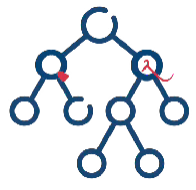
\includegraphics[height=0.9cm]{msca_logo.png}}%
  \end{center}
  \vspace{0.45cm}
  \begin{center}
    \begin{minipage}{0.1\textwidth}\centering
      \href{https://quantlet.com}{
\includegraphics[height=0.9cm]{ql_logo.png}}\end{minipage}%
    \begin{minipage}{0.78\textwidth}\centering
      {\Large\bfseries\usebeamercolor[fg]{title}\inserttitle}\par\vspace{0.25cm}
      {\large\usebeamercolor[fg]{title}\insertsubtitle}\end{minipage}%
    \begin{minipage}{0.1\textwidth}\centering
      \href{https://quantinar.com}{
\includegraphics[height=0.9cm]{qr_logo.png}}\end{minipage}
  \end{center}
  \vfill
  \hspace{0.4cm}{\bfseries\insertauthor}\par\vspace{0.12cm}
  \hspace{0.4cm}\begin{minipage}[t]{0.92\textwidth}\raggedright\footnotesize\insertinstitute\end{minipage}
  \par\vspace{0.4cm}}

% ---------------------------------------------------------------- lecture metadata
\newcommand{\nnshort}{}
\newcommand{\nnnb}{notebooks}
\newcommand{\nnrepo}{https://github.com/danpele/NEURAL_BIZ/tree/main}
% language-dependent labels (English default; \nnromanian switches to Romanian, call it before \nnlecture)
\newcommand{\txtcourse}{Neural Networks and Deep Learning}
\newcommand{\txtlecture}{Lecture}
\newcommand{\txtoutline}{Outline}
\newcommand{\txtintuition}{In one sentence:}
\newcommand{\txtjob}{In practice:}
\newcommand{\txttry}{Experiment yourself:}
\newcommand{\txtwhere}{where}
\newcommand{\txtsim}{SIMULATED DATA (teaching illustration)}
\newcommand{\txtnbsuffix}{}
\newcommand{\txtinstitute}{Bucharest University of Economic Studies (ASE), Department of Statistics and Econometrics\\
    Romanian Academy, Institute for Economic Forecasting (IPE)\\
    IDA Institute Digital Assets \textbullet\ AI4EFin \textbullet\ MSCA Digital Finance}
\newcommand{\nnromanian}{%
  \renewcommand{\txtcourse}{Rețele neuronale și deep learning}%
  \renewcommand{\txtlecture}{Cursul}%
  \renewcommand{\txtoutline}{Cuprins}%
  \renewcommand{\txtintuition}{Pe scurt:}%
  \renewcommand{\txtjob}{În practică:}%
  \renewcommand{\txttry}{Exercițiu practic:}%
  \renewcommand{\txtwhere}{unde}%
  \renewcommand{\txtsim}{DATE SIMULATE (doar pentru ilustrare)}%
  \renewcommand{\txtnbsuffix}{\string_ro}%
  \renewcommand{\txtinstitute}{Academia de Studii Economice din București (ASE), Departamentul de Statistică și Econometrie\\
    Academia Română, Institutul de Prognoză Economică (IPE)\\
    IDA Institute Digital Assets \textbullet\ AI4EFin \textbullet\ MSCA Digital Finance}}
\newcommand{\nnlecture}[2]{%
  \renewcommand{\nnshort}{\txtlecture\ #1}%
  \renewcommand{\nnnb}{notebooks/L#1\string_notebook\txtnbsuffix.ipynb}%
  \title[NN]{\txtcourse}%
  \subtitle{\txtlecture\ #1: #2}%
  \author{Prof.\ dr.\ Daniel Traian PELE}%
  \institute{\txtinstitute}%
  \date{}}

% ---------------------------------------------------------------- teaching blocks (one message per frame)
% \intuition{one plain sentence}  ->  formula with every symbol defined  ->  real-data example  ->  \manager{one line}
\newcommand{\intuition}[1]{\begin{itemize}\item {\color{MainBlue}\textbf{\txtintuition}}~#1\end{itemize}\vspace{0.6mm}}
\newcommand{\manager}[1]{\colorbox{Forest!10}{\parbox{\dimexpr\linewidth-2\fboxsep\relax}{\footnotesize
  \begin{itemize}\setlength{\itemsep}{0pt}\item \textbf{\color{Forest}\txtjob}~#1\end{itemize}}}}
% Experiment yourself: pointer to the matching notebook section
\newcommand{\tryit}[1]{{\scriptsize\href{\nnrepo/\nnnb}{%
  \raisebox{-0.15em}{
\includegraphics[height=0.85em]{ql_logo.png}}\,\textbf{\txttry}~\color{MainBlue}#1}}}
% bottom row: manager line (left) + experiment pointer (right), pinned to the bottom of the frame
\newcommand{\bottomrow}[2]{\par\vfill\noindent\begin{minipage}[b]{0.72\linewidth}#1\end{minipage}\hfill
  \begin{minipage}[b]{0.26\linewidth}\raggedleft #2\end{minipage}\par\vspace{0.5mm}}
\newcommand{\where}[1]{{\footnotesize\textbf{\txtwhere}~#1\par}}

% ---------------------------------------------------------------- helpers
% chart source line under a figure: \chartsource{Source ...; period ...}
\newcommand{\chartsource}[1]{\par\vspace{1pt}{\scriptsize\color{FooterGray}#1\par}}
% link to code: \quantlet{label}{path inside the repo}
\newcommand{\quantlet}[2]{\par\vspace{1pt}\hfill\href{\nnrepo/#2}{%
  \raisebox{-0.15em}{
\includegraphics[height=0.75em]{ql_logo.png}}\textcolor{MainBlue}{\scriptsize\ #1}}}
% inline Quantlet link for the bottom-right corner of a frame: \qlink{label}{path inside the repo}
\newcommand{\qlink}[2]{{\scriptsize\href{\nnrepo/#2}{\raisebox{-0.15em}{
\includegraphics[height=0.85em]{ql_logo.png}}\,\textcolor{MainBlue}{#1}}}}
\newcommand{\simlabel}{\colorbox{Crimson!12}{\scriptsize\bfseries\color{Crimson}\txtsim}}
\newcommand{\E}{\mathbb{E}}
\newcommand{\Var}{\operatorname{Var}}
\newcommand{\Cov}{\operatorname{Cov}}
\newcommand{\Corr}{\operatorname{Corr}}
\newcommand{\asinh}{\operatorname{asinh}}
\newcommand{\iid}{\overset{\text{i.i.d.}}{\sim}}
\newcommand{\EUR}{EUR}
% deep-learning notation (Bishop & Bishop, 2024): vectors bold lower case, matrices bold upper case
\newcommand{\R}{\mathbb{R}}
\newcommand{\vx}{\mathbf{x}}
\newcommand{\vy}{\mathbf{y}}
\newcommand{\vz}{\mathbf{z}}
\newcommand{\vh}{\mathbf{h}}
\newcommand{\vw}{\mathbf{w}}
\newcommand{\vb}{\mathbf{b}}
\newcommand{\mW}{\mathbf{W}}
\newcommand{\mX}{\mathbf{X}}
\newcommand{\btheta}{\boldsymbol{\theta}}
\newcommand{\loss}{\mathcal{L}}
\newcommand{\dataset}{\mathcal{D}}
\DeclareMathOperator*{\argmin}{arg\,min}
\DeclareMathOperator*{\argmax}{arg\,max}
\DeclareMathOperator{\softmax}{softmax}
\DeclareMathOperator{\ReLU}{ReLU}
\DeclareMathOperator{\sigm}{\sigma}

%   \nnlecture{k}{Lecture title}
% Logos live in lectures/common/logos/, charts in lectures/Lk/charts/.
% Do NOT add \hfuzz / \vfuzz / \hbadness here: overfull boxes must be fixed, not hidden.
% =============================================================================

\usetheme{default}
\setbeamersize{text margin left=7mm, text margin right=7mm}

% ---------------------------------------------------------------- packages
\usepackage[utf8]{inputenc}
\usepackage[T1]{fontenc}
\usepackage{lmodern}
\usepackage{amsmath, amssymb}
\usepackage{mathtools}
\usepackage{bm}
\usepackage{tikz}
\usetikzlibrary{arrows.meta, positioning, calc, shapes.misc}
\usepackage{booktabs}
\usepackage{array}
\usepackage{graphicx}
\usepackage{colortbl}
\usepackage{xcolor}
\usepackage{multicol}
\hypersetup{colorlinks=true, linkcolor=MainBlue, urlcolor=MainBlue, citecolor=MainBlue}
\graphicspath{{../common/logos/}}   % charts are included with their language folder: charts/en/, charts/ro/

% ---------------------------------------------------------------- colours
\definecolor{MainBlue}{RGB}{26, 58, 110}
\definecolor{IDAred}{RGB}{205, 0, 0}
\definecolor{DarkGray}{RGB}{51, 51, 51}
\definecolor{FooterGray}{RGB}{100, 100, 100}
\definecolor{BlockGray}{RGB}{236, 238, 242}
\definecolor{KeynoteGray}{RGB}{218, 218, 218}
\definecolor{Crimson}{RGB}{190, 40, 50}
\definecolor{Forest}{RGB}{30, 110, 50}
\definecolor{Bitter}{RGB}{214, 150, 20}
% chart palette (same hex values and order as lectures/common/nn_plot.py SERIES)
\definecolor{Ser1}{HTML}{2A78D6}
\definecolor{Ser2}{HTML}{EB6834}
\definecolor{Ser3}{HTML}{1BAF7A}
\definecolor{Ser4}{HTML}{EDA100}
\definecolor{Ser5}{HTML}{E87BA4}
\definecolor{Ser6}{HTML}{008300}
\definecolor{Ser7}{HTML}{6250D6}
\definecolor{Ser8}{HTML}{E34948}

\setbeamertemplate{background}{%
  \begin{tikzpicture}[remember picture, overlay]
    \shade[shading=axis, shading angle=315, top color=white, bottom color=KeynoteGray]
      (current page.south west) rectangle (current page.north east);
  \end{tikzpicture}}
\setbeamercolor{background canvas}{bg=}
\setbeamercolor{structure}{fg=MainBlue}
\setbeamercolor{normal text}{fg=DarkGray}
\setbeamercolor{title}{fg=IDAred}
\setbeamercolor{frametitle}{fg=IDAred, bg=}
\setbeamercolor{block title}{bg=MainBlue, fg=white}
\setbeamercolor{block body}{bg=BlockGray, fg=DarkGray}
\setbeamercolor{block title alerted}{bg=Crimson, fg=white}
\setbeamercolor{block body alerted}{bg=Crimson!7, fg=DarkGray}
\setbeamercolor{block title example}{bg=Forest, fg=white}
\setbeamercolor{block body example}{bg=Forest!7, fg=DarkGray}
\setbeamercolor{item}{fg=MainBlue}
\setbeamerfont{frametitle}{size=\large, series=\bfseries}
\setbeamerfont{block title}{size=\small, series=\bfseries}
\setbeamertemplate{blocks}[rounded][shadow=false]
\setbeamertemplate{itemize item}{\color{MainBlue}$\boxdot$}
\setbeamertemplate{itemize subitem}{\color{MainBlue}\scriptsize$\blacktriangleright$}
% compact two-level lists: level 1 = main point, level 2 = details (no text outside bullets)
\setbeamerfont{itemize/enumerate subbody}{size=\footnotesize}
\setlength{\leftmargini}{1.1em}
\setlength{\leftmarginii}{1.1em}
\setbeamertemplate{itemize/enumerate body begin}{\setlength{\topsep}{0pt}\setlength{\partopsep}{0pt}\setlength{\parskip}{0pt}}
\setbeamertemplate{itemize/enumerate subbody begin}{\setlength{\topsep}{0pt}\setlength{\partopsep}{0pt}\setlength{\itemsep}{0pt}\vspace{-0.4ex}}

\setbeamertemplate{enumerate item}{\color{MainBlue}\insertenumlabel.}
\setlength{\leftmargini}{1.3em}
\setlength{\leftmarginii}{1.2em}
\setbeamertemplate{navigation symbols}{}
\setbeamertemplate{section in toc}{\color{MainBlue}$\blacktriangleright$~\inserttocsection}
\setbeamertemplate{caption}{\raggedright\insertcaption\par}
% frame subtitle = precise citation line under the claim title (Weron style)
\setbeamerfont{framesubtitle}{size=\footnotesize}
\setbeamercolor{framesubtitle}{fg=FooterGray}
% outline that reappears at every section with the current section highlighted
\setbeamertemplate{section in toc shaded}[default][35]
\setbeamertemplate{subsection in toc shaded}[default][35]
\setbeamertemplate{subsection in toc}{\leavevmode\leftskip=2.2em\color{DarkGray}\small\inserttocsubsection\par}
\AtBeginSection[]{{\begin{frame}{\txtoutline}\vspace{2mm}\small
  \tableofcontents[currentsection,hideothersubsections]\end{frame}}}

% ---------------------------------------------------------------- head and foot
\setbeamertemplate{headline}{%
  \vskip10pt%
  \hbox to \paperwidth{\hskip0.5cm%
    {\small\color{FooterGray}\renewcommand{\hyperlink}[2]{##2}\insertsectionhead}%
    \hfill\textcolor{FooterGray}{\small\insertframenumber}\hskip0.5cm}%
  \vskip4pt{\color{FooterGray}\hrule height 0.4pt}}
% footer as in the other courses (MFM, SFM): course name on the left, small sparkline on the right
\setbeamertemplate{footline}{%
  {\color{FooterGray}\hrule height 0.4pt}\vskip4pt%
  \hbox to \paperwidth{\hskip0.5cm%
    \textcolor{FooterGray}{\small\txtcourse}%
    \hfill\raisebox{-0.1em}{\begin{tikzpicture}[x=0.08em, y=0.08em, line width=0.4pt]
      \draw[FooterGray] (0,3) -- (1,4) -- (2,3.5) -- (3,5) -- (4,4) -- (5,6) -- (6,5.5) -- (7,4) -- (8,5) -- (9,7) -- (10,6) -- (11,5) -- (12,6.5) -- (13,8) -- (14,7) -- (15,6) -- (16,7.5) -- (17,9) -- (18,8) -- (19,7) -- (20,8.5) -- (21,10) -- (22,9) -- (23,8) -- (24,9.5);
    \end{tikzpicture}}\hskip0.5cm}%
  \vskip6pt}

% ---------------------------------------------------------------- title page
\defbeamertemplate*{title page}{nn}[1][]{%
  \vspace{0.15cm}
  \begin{center}
    \href{https://www.ase.ro}{
\includegraphics[height=0.9cm]{ase_logo.png}}\hspace{0.3cm}%
    \href{https://ipe.ro/new}{
\includegraphics[height=0.9cm]{acad_logo.png}}\hspace{0.3cm}%
    \href{https://theida.net}{
\includegraphics[height=0.9cm]{ida_logo.png}}\hspace{0.3cm}%
    \href{https://blockchain-research-center.com}{
\includegraphics[height=0.9cm]{brc_logo.png}}\hspace{0.3cm}%
    \href{https://www.ai4efin.ase.ro}{
\includegraphics[height=0.9cm]{ai4efin_logo.png}}\hspace{0.3cm}%
    \href{https://www.digital-finance-msca.com}{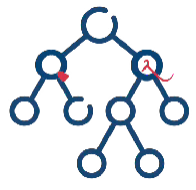
\includegraphics[height=0.9cm]{msca_logo.png}}%
  \end{center}
  \vspace{0.45cm}
  \begin{center}
    \begin{minipage}{0.1\textwidth}\centering
      \href{https://quantlet.com}{
\includegraphics[height=0.9cm]{ql_logo.png}}\end{minipage}%
    \begin{minipage}{0.78\textwidth}\centering
      {\Large\bfseries\usebeamercolor[fg]{title}\inserttitle}\par\vspace{0.25cm}
      {\large\usebeamercolor[fg]{title}\insertsubtitle}\end{minipage}%
    \begin{minipage}{0.1\textwidth}\centering
      \href{https://quantinar.com}{
\includegraphics[height=0.9cm]{qr_logo.png}}\end{minipage}
  \end{center}
  \vfill
  \hspace{0.4cm}{\bfseries\insertauthor}\par\vspace{0.12cm}
  \hspace{0.4cm}\begin{minipage}[t]{0.92\textwidth}\raggedright\footnotesize\insertinstitute\end{minipage}
  \par\vspace{0.4cm}}

% ---------------------------------------------------------------- lecture metadata
\newcommand{\nnshort}{}
\newcommand{\nnnb}{notebooks}
\newcommand{\nnrepo}{https://github.com/danpele/NEURAL_BIZ/tree/main}
% language-dependent labels (English default; \nnromanian switches to Romanian, call it before \nnlecture)
\newcommand{\txtcourse}{Neural Networks and Deep Learning}
\newcommand{\txtlecture}{Lecture}
\newcommand{\txtoutline}{Outline}
\newcommand{\txtintuition}{In one sentence:}
\newcommand{\txtjob}{In practice:}
\newcommand{\txttry}{Experiment yourself:}
\newcommand{\txtwhere}{where}
\newcommand{\txtsim}{SIMULATED DATA (teaching illustration)}
\newcommand{\txtnbsuffix}{}
\newcommand{\txtinstitute}{Bucharest University of Economic Studies (ASE), Department of Statistics and Econometrics\\
    Romanian Academy, Institute for Economic Forecasting (IPE)\\
    IDA Institute Digital Assets \textbullet\ AI4EFin \textbullet\ MSCA Digital Finance}
\newcommand{\nnromanian}{%
  \renewcommand{\txtcourse}{Rețele neuronale și deep learning}%
  \renewcommand{\txtlecture}{Cursul}%
  \renewcommand{\txtoutline}{Cuprins}%
  \renewcommand{\txtintuition}{Pe scurt:}%
  \renewcommand{\txtjob}{În practică:}%
  \renewcommand{\txttry}{Exercițiu practic:}%
  \renewcommand{\txtwhere}{unde}%
  \renewcommand{\txtsim}{DATE SIMULATE (doar pentru ilustrare)}%
  \renewcommand{\txtnbsuffix}{\string_ro}%
  \renewcommand{\txtinstitute}{Academia de Studii Economice din București (ASE), Departamentul de Statistică și Econometrie\\
    Academia Română, Institutul de Prognoză Economică (IPE)\\
    IDA Institute Digital Assets \textbullet\ AI4EFin \textbullet\ MSCA Digital Finance}}
\newcommand{\nnlecture}[2]{%
  \renewcommand{\nnshort}{\txtlecture\ #1}%
  \renewcommand{\nnnb}{notebooks/L#1\string_notebook\txtnbsuffix.ipynb}%
  \title[NN]{\txtcourse}%
  \subtitle{\txtlecture\ #1: #2}%
  \author{Prof.\ dr.\ Daniel Traian PELE}%
  \institute{\txtinstitute}%
  \date{}}

% ---------------------------------------------------------------- teaching blocks (one message per frame)
% \intuition{one plain sentence}  ->  formula with every symbol defined  ->  real-data example  ->  \manager{one line}
\newcommand{\intuition}[1]{\begin{itemize}\item {\color{MainBlue}\textbf{\txtintuition}}~#1\end{itemize}\vspace{0.6mm}}
\newcommand{\manager}[1]{\colorbox{Forest!10}{\parbox{\dimexpr\linewidth-2\fboxsep\relax}{\footnotesize
  \begin{itemize}\setlength{\itemsep}{0pt}\item \textbf{\color{Forest}\txtjob}~#1\end{itemize}}}}
% Experiment yourself: pointer to the matching notebook section
\newcommand{\tryit}[1]{{\scriptsize\href{\nnrepo/\nnnb}{%
  \raisebox{-0.15em}{
\includegraphics[height=0.85em]{ql_logo.png}}\,\textbf{\txttry}~\color{MainBlue}#1}}}
% bottom row: manager line (left) + experiment pointer (right), pinned to the bottom of the frame
\newcommand{\bottomrow}[2]{\par\vfill\noindent\begin{minipage}[b]{0.72\linewidth}#1\end{minipage}\hfill
  \begin{minipage}[b]{0.26\linewidth}\raggedleft #2\end{minipage}\par\vspace{0.5mm}}
\newcommand{\where}[1]{{\footnotesize\textbf{\txtwhere}~#1\par}}

% ---------------------------------------------------------------- helpers
% chart source line under a figure: \chartsource{Source ...; period ...}
\newcommand{\chartsource}[1]{\par\vspace{1pt}{\scriptsize\color{FooterGray}#1\par}}
% link to code: \quantlet{label}{path inside the repo}
\newcommand{\quantlet}[2]{\par\vspace{1pt}\hfill\href{\nnrepo/#2}{%
  \raisebox{-0.15em}{
\includegraphics[height=0.75em]{ql_logo.png}}\textcolor{MainBlue}{\scriptsize\ #1}}}
% inline Quantlet link for the bottom-right corner of a frame: \qlink{label}{path inside the repo}
\newcommand{\qlink}[2]{{\scriptsize\href{\nnrepo/#2}{\raisebox{-0.15em}{
\includegraphics[height=0.85em]{ql_logo.png}}\,\textcolor{MainBlue}{#1}}}}
\newcommand{\simlabel}{\colorbox{Crimson!12}{\scriptsize\bfseries\color{Crimson}\txtsim}}
\newcommand{\E}{\mathbb{E}}
\newcommand{\Var}{\operatorname{Var}}
\newcommand{\Cov}{\operatorname{Cov}}
\newcommand{\Corr}{\operatorname{Corr}}
\newcommand{\asinh}{\operatorname{asinh}}
\newcommand{\iid}{\overset{\text{i.i.d.}}{\sim}}
\newcommand{\EUR}{EUR}
% deep-learning notation (Bishop & Bishop, 2024): vectors bold lower case, matrices bold upper case
\newcommand{\R}{\mathbb{R}}
\newcommand{\vx}{\mathbf{x}}
\newcommand{\vy}{\mathbf{y}}
\newcommand{\vz}{\mathbf{z}}
\newcommand{\vh}{\mathbf{h}}
\newcommand{\vw}{\mathbf{w}}
\newcommand{\vb}{\mathbf{b}}
\newcommand{\mW}{\mathbf{W}}
\newcommand{\mX}{\mathbf{X}}
\newcommand{\btheta}{\boldsymbol{\theta}}
\newcommand{\loss}{\mathcal{L}}
\newcommand{\dataset}{\mathcal{D}}
\DeclareMathOperator*{\argmin}{arg\,min}
\DeclareMathOperator*{\argmax}{arg\,max}
\DeclareMathOperator{\softmax}{softmax}
\DeclareMathOperator{\ReLU}{ReLU}
\DeclareMathOperator{\sigm}{\sigma}

%   \nnlecture{k}{Lecture title}
% Logos live in lectures/common/logos/, charts in lectures/Lk/charts/.
% Do NOT add \hfuzz / \vfuzz / \hbadness here: overfull boxes must be fixed, not hidden.
% =============================================================================

\usetheme{default}
\setbeamersize{text margin left=7mm, text margin right=7mm}

% ---------------------------------------------------------------- packages
\usepackage[utf8]{inputenc}
\usepackage[T1]{fontenc}
\usepackage{lmodern}
\usepackage{amsmath, amssymb}
\usepackage{mathtools}
\usepackage{bm}
\usepackage{tikz}
\usetikzlibrary{arrows.meta, positioning, calc, shapes.misc}
\usepackage{booktabs}
\usepackage{array}
\usepackage{graphicx}
\usepackage{colortbl}
\usepackage{xcolor}
\usepackage{multicol}
\hypersetup{colorlinks=true, linkcolor=MainBlue, urlcolor=MainBlue, citecolor=MainBlue}
\graphicspath{{../common/logos/}}   % charts are included with their language folder: charts/en/, charts/ro/

% ---------------------------------------------------------------- colours
\definecolor{MainBlue}{RGB}{26, 58, 110}
\definecolor{IDAred}{RGB}{205, 0, 0}
\definecolor{DarkGray}{RGB}{51, 51, 51}
\definecolor{FooterGray}{RGB}{100, 100, 100}
\definecolor{BlockGray}{RGB}{236, 238, 242}
\definecolor{KeynoteGray}{RGB}{218, 218, 218}
\definecolor{Crimson}{RGB}{190, 40, 50}
\definecolor{Forest}{RGB}{30, 110, 50}
\definecolor{Bitter}{RGB}{214, 150, 20}
% chart palette (same hex values and order as lectures/common/nn_plot.py SERIES)
\definecolor{Ser1}{HTML}{2A78D6}
\definecolor{Ser2}{HTML}{EB6834}
\definecolor{Ser3}{HTML}{1BAF7A}
\definecolor{Ser4}{HTML}{EDA100}
\definecolor{Ser5}{HTML}{E87BA4}
\definecolor{Ser6}{HTML}{008300}
\definecolor{Ser7}{HTML}{6250D6}
\definecolor{Ser8}{HTML}{E34948}

\setbeamertemplate{background}{%
  \begin{tikzpicture}[remember picture, overlay]
    \shade[shading=axis, shading angle=315, top color=white, bottom color=KeynoteGray]
      (current page.south west) rectangle (current page.north east);
  \end{tikzpicture}}
\setbeamercolor{background canvas}{bg=}
\setbeamercolor{structure}{fg=MainBlue}
\setbeamercolor{normal text}{fg=DarkGray}
\setbeamercolor{title}{fg=IDAred}
\setbeamercolor{frametitle}{fg=IDAred, bg=}
\setbeamercolor{block title}{bg=MainBlue, fg=white}
\setbeamercolor{block body}{bg=BlockGray, fg=DarkGray}
\setbeamercolor{block title alerted}{bg=Crimson, fg=white}
\setbeamercolor{block body alerted}{bg=Crimson!7, fg=DarkGray}
\setbeamercolor{block title example}{bg=Forest, fg=white}
\setbeamercolor{block body example}{bg=Forest!7, fg=DarkGray}
\setbeamercolor{item}{fg=MainBlue}
\setbeamerfont{frametitle}{size=\large, series=\bfseries}
\setbeamerfont{block title}{size=\small, series=\bfseries}
\setbeamertemplate{blocks}[rounded][shadow=false]
\setbeamertemplate{itemize item}{\color{MainBlue}$\boxdot$}
\setbeamertemplate{itemize subitem}{\color{MainBlue}\scriptsize$\blacktriangleright$}
% compact two-level lists: level 1 = main point, level 2 = details (no text outside bullets)
\setbeamerfont{itemize/enumerate subbody}{size=\footnotesize}
\setlength{\leftmargini}{1.1em}
\setlength{\leftmarginii}{1.1em}
\setbeamertemplate{itemize/enumerate body begin}{\setlength{\topsep}{0pt}\setlength{\partopsep}{0pt}\setlength{\parskip}{0pt}}
\setbeamertemplate{itemize/enumerate subbody begin}{\setlength{\topsep}{0pt}\setlength{\partopsep}{0pt}\setlength{\itemsep}{0pt}\vspace{-0.4ex}}

\setbeamertemplate{enumerate item}{\color{MainBlue}\insertenumlabel.}
\setlength{\leftmargini}{1.3em}
\setlength{\leftmarginii}{1.2em}
\setbeamertemplate{navigation symbols}{}
\setbeamertemplate{section in toc}{\color{MainBlue}$\blacktriangleright$~\inserttocsection}
\setbeamertemplate{caption}{\raggedright\insertcaption\par}
% frame subtitle = precise citation line under the claim title (Weron style)
\setbeamerfont{framesubtitle}{size=\footnotesize}
\setbeamercolor{framesubtitle}{fg=FooterGray}
% outline that reappears at every section with the current section highlighted
\setbeamertemplate{section in toc shaded}[default][35]
\setbeamertemplate{subsection in toc shaded}[default][35]
\setbeamertemplate{subsection in toc}{\leavevmode\leftskip=2.2em\color{DarkGray}\small\inserttocsubsection\par}
\AtBeginSection[]{{\begin{frame}{\txtoutline}\vspace{2mm}\small
  \tableofcontents[currentsection,hideothersubsections]\end{frame}}}

% ---------------------------------------------------------------- head and foot
\setbeamertemplate{headline}{%
  \vskip10pt%
  \hbox to \paperwidth{\hskip0.5cm%
    {\small\color{FooterGray}\renewcommand{\hyperlink}[2]{##2}\insertsectionhead}%
    \hfill\textcolor{FooterGray}{\small\insertframenumber}\hskip0.5cm}%
  \vskip4pt{\color{FooterGray}\hrule height 0.4pt}}
% footer as in the other courses (MFM, SFM): course name on the left, small sparkline on the right
\setbeamertemplate{footline}{%
  {\color{FooterGray}\hrule height 0.4pt}\vskip4pt%
  \hbox to \paperwidth{\hskip0.5cm%
    \textcolor{FooterGray}{\small\txtcourse}%
    \hfill\raisebox{-0.1em}{\begin{tikzpicture}[x=0.08em, y=0.08em, line width=0.4pt]
      \draw[FooterGray] (0,3) -- (1,4) -- (2,3.5) -- (3,5) -- (4,4) -- (5,6) -- (6,5.5) -- (7,4) -- (8,5) -- (9,7) -- (10,6) -- (11,5) -- (12,6.5) -- (13,8) -- (14,7) -- (15,6) -- (16,7.5) -- (17,9) -- (18,8) -- (19,7) -- (20,8.5) -- (21,10) -- (22,9) -- (23,8) -- (24,9.5);
    \end{tikzpicture}}\hskip0.5cm}%
  \vskip6pt}

% ---------------------------------------------------------------- title page
\defbeamertemplate*{title page}{nn}[1][]{%
  \vspace{0.15cm}
  \begin{center}
    \href{https://www.ase.ro}{
\includegraphics[height=0.9cm]{ase_logo.png}}\hspace{0.3cm}%
    \href{https://ipe.ro/new}{
\includegraphics[height=0.9cm]{acad_logo.png}}\hspace{0.3cm}%
    \href{https://theida.net}{
\includegraphics[height=0.9cm]{ida_logo.png}}\hspace{0.3cm}%
    \href{https://blockchain-research-center.com}{
\includegraphics[height=0.9cm]{brc_logo.png}}\hspace{0.3cm}%
    \href{https://www.ai4efin.ase.ro}{
\includegraphics[height=0.9cm]{ai4efin_logo.png}}\hspace{0.3cm}%
    \href{https://www.digital-finance-msca.com}{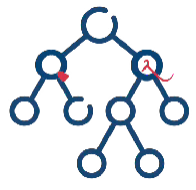
\includegraphics[height=0.9cm]{msca_logo.png}}%
  \end{center}
  \vspace{0.45cm}
  \begin{center}
    \begin{minipage}{0.1\textwidth}\centering
      \href{https://quantlet.com}{
\includegraphics[height=0.9cm]{ql_logo.png}}\end{minipage}%
    \begin{minipage}{0.78\textwidth}\centering
      {\Large\bfseries\usebeamercolor[fg]{title}\inserttitle}\par\vspace{0.25cm}
      {\large\usebeamercolor[fg]{title}\insertsubtitle}\end{minipage}%
    \begin{minipage}{0.1\textwidth}\centering
      \href{https://quantinar.com}{
\includegraphics[height=0.9cm]{qr_logo.png}}\end{minipage}
  \end{center}
  \vfill
  \hspace{0.4cm}{\bfseries\insertauthor}\par\vspace{0.12cm}
  \hspace{0.4cm}\begin{minipage}[t]{0.92\textwidth}\raggedright\footnotesize\insertinstitute\end{minipage}
  \par\vspace{0.4cm}}

% ---------------------------------------------------------------- lecture metadata
\newcommand{\nnshort}{}
\newcommand{\nnnb}{notebooks}
\newcommand{\nnrepo}{https://github.com/danpele/NEURAL_BIZ/tree/main}
% language-dependent labels (English default; \nnromanian switches to Romanian, call it before \nnlecture)
\newcommand{\txtcourse}{Neural Networks and Deep Learning}
\newcommand{\txtlecture}{Lecture}
\newcommand{\txtoutline}{Outline}
\newcommand{\txtintuition}{In one sentence:}
\newcommand{\txtjob}{In practice:}
\newcommand{\txttry}{Experiment yourself:}
\newcommand{\txtwhere}{where}
\newcommand{\txtsim}{SIMULATED DATA (teaching illustration)}
\newcommand{\txtnbsuffix}{}
\newcommand{\txtinstitute}{Bucharest University of Economic Studies (ASE), Department of Statistics and Econometrics\\
    Romanian Academy, Institute for Economic Forecasting (IPE)\\
    IDA Institute Digital Assets \textbullet\ AI4EFin \textbullet\ MSCA Digital Finance}
\newcommand{\nnromanian}{%
  \renewcommand{\txtcourse}{Rețele neuronale și deep learning}%
  \renewcommand{\txtlecture}{Cursul}%
  \renewcommand{\txtoutline}{Cuprins}%
  \renewcommand{\txtintuition}{Pe scurt:}%
  \renewcommand{\txtjob}{În practică:}%
  \renewcommand{\txttry}{Exercițiu practic:}%
  \renewcommand{\txtwhere}{unde}%
  \renewcommand{\txtsim}{DATE SIMULATE (doar pentru ilustrare)}%
  \renewcommand{\txtnbsuffix}{\string_ro}%
  \renewcommand{\txtinstitute}{Academia de Studii Economice din București (ASE), Departamentul de Statistică și Econometrie\\
    Academia Română, Institutul de Prognoză Economică (IPE)\\
    IDA Institute Digital Assets \textbullet\ AI4EFin \textbullet\ MSCA Digital Finance}}
\newcommand{\nnlecture}[2]{%
  \renewcommand{\nnshort}{\txtlecture\ #1}%
  \renewcommand{\nnnb}{notebooks/L#1\string_notebook\txtnbsuffix.ipynb}%
  \title[NN]{\txtcourse}%
  \subtitle{\txtlecture\ #1: #2}%
  \author{Prof.\ dr.\ Daniel Traian PELE}%
  \institute{\txtinstitute}%
  \date{}}

% ---------------------------------------------------------------- teaching blocks (one message per frame)
% \intuition{one plain sentence}  ->  formula with every symbol defined  ->  real-data example  ->  \manager{one line}
\newcommand{\intuition}[1]{\begin{itemize}\item {\color{MainBlue}\textbf{\txtintuition}}~#1\end{itemize}\vspace{0.6mm}}
\newcommand{\manager}[1]{\colorbox{Forest!10}{\parbox{\dimexpr\linewidth-2\fboxsep\relax}{\footnotesize
  \begin{itemize}\setlength{\itemsep}{0pt}\item \textbf{\color{Forest}\txtjob}~#1\end{itemize}}}}
% Experiment yourself: pointer to the matching notebook section
\newcommand{\tryit}[1]{{\scriptsize\href{\nnrepo/\nnnb}{%
  \raisebox{-0.15em}{
\includegraphics[height=0.85em]{ql_logo.png}}\,\textbf{\txttry}~\color{MainBlue}#1}}}
% bottom row: manager line (left) + experiment pointer (right), pinned to the bottom of the frame
\newcommand{\bottomrow}[2]{\par\vfill\noindent\begin{minipage}[b]{0.72\linewidth}#1\end{minipage}\hfill
  \begin{minipage}[b]{0.26\linewidth}\raggedleft #2\end{minipage}\par\vspace{0.5mm}}
\newcommand{\where}[1]{{\footnotesize\textbf{\txtwhere}~#1\par}}

% ---------------------------------------------------------------- helpers
% chart source line under a figure: \chartsource{Source ...; period ...}
\newcommand{\chartsource}[1]{\par\vspace{1pt}{\scriptsize\color{FooterGray}#1\par}}
% link to code: \quantlet{label}{path inside the repo}
\newcommand{\quantlet}[2]{\par\vspace{1pt}\hfill\href{\nnrepo/#2}{%
  \raisebox{-0.15em}{
\includegraphics[height=0.75em]{ql_logo.png}}\textcolor{MainBlue}{\scriptsize\ #1}}}
% inline Quantlet link for the bottom-right corner of a frame: \qlink{label}{path inside the repo}
\newcommand{\qlink}[2]{{\scriptsize\href{\nnrepo/#2}{\raisebox{-0.15em}{
\includegraphics[height=0.85em]{ql_logo.png}}\,\textcolor{MainBlue}{#1}}}}
\newcommand{\simlabel}{\colorbox{Crimson!12}{\scriptsize\bfseries\color{Crimson}\txtsim}}
\newcommand{\E}{\mathbb{E}}
\newcommand{\Var}{\operatorname{Var}}
\newcommand{\Cov}{\operatorname{Cov}}
\newcommand{\Corr}{\operatorname{Corr}}
\newcommand{\asinh}{\operatorname{asinh}}
\newcommand{\iid}{\overset{\text{i.i.d.}}{\sim}}
\newcommand{\EUR}{EUR}
% deep-learning notation (Bishop & Bishop, 2024): vectors bold lower case, matrices bold upper case
\newcommand{\R}{\mathbb{R}}
\newcommand{\vx}{\mathbf{x}}
\newcommand{\vy}{\mathbf{y}}
\newcommand{\vz}{\mathbf{z}}
\newcommand{\vh}{\mathbf{h}}
\newcommand{\vw}{\mathbf{w}}
\newcommand{\vb}{\mathbf{b}}
\newcommand{\mW}{\mathbf{W}}
\newcommand{\mX}{\mathbf{X}}
\newcommand{\btheta}{\boldsymbol{\theta}}
\newcommand{\loss}{\mathcal{L}}
\newcommand{\dataset}{\mathcal{D}}
\DeclareMathOperator*{\argmin}{arg\,min}
\DeclareMathOperator*{\argmax}{arg\,max}
\DeclareMathOperator{\softmax}{softmax}
\DeclareMathOperator{\ReLU}{ReLU}
\DeclareMathOperator{\sigm}{\sigma}

\nnlecture{11}{Explainable AI: SHAP, LIME, gradient methods and the stability of explanations}
\begin{document}
{\setbeamertemplate{headline}{}\setbeamertemplate{footline}{}
\begin{frame}\titlepage\end{frame}}
% END-FRONT-MATTER

\begin{frame}{Learning objectives}
\small
\begin{itemize}\setlength{\itemsep}{4pt}
  \item Explain why banks, insurers and regulators require explanations of a neural network, and classify explanation methods of explainable artificial intelligence (XAI).
  \item Compute Shapley additive explanations (SHAP) and local interpretable model-agnostic explanations (LIME) with full formulas, and read them for one customer and for a portfolio.
  \item Use gradient methods (saliency, integrated gradients, SmoothGrad) and check their axioms on a real fraud model.
  \item Test whether explanations agree, are faithful to the model and stay stable across seeds, samples and time.
  \item Write a counterfactual explanation that a rejected applicant can act on.
\end{itemize}
\end{frame}

% BEGIN-ABBR

\begin{frame}{Abbreviations}
\small
\vspace{-1mm}\begin{columns}[T,onlytextwidth]
\begin{column}{0.49\textwidth}{\scriptsize\renewcommand{\arraystretch}{0.96}\begin{tabular}{@{}>{\bfseries}l@{\ \ }p{0.74\linewidth}@{}}AI & artificial intelligence\\
AOPC & area over the perturbation curve\\
ASE & Bucharest University of Economic Studies\\
AUC & area under the ROC curve\\
EBA & European Banking Authority\\
EU & European Union\\
EUR & euro\\
GDPR & General Data Protection Regulation\\
GNN & graph neural network\\
HMEQ & home-equity loan data set\\
ICE & individual conditional expectation\\
IG & integrated gradients\\
IPE & Institute for Economic Forecasting, Romanian Academy\\
JS & Jensen-Shannon divergence\\
KL & Kullback-Leibler divergence\\
LIME & local interpretable model-agnostic explanations\\\end{tabular}}\end{column}
\begin{column}{0.49\textwidth}{\scriptsize\renewcommand{\arraystretch}{0.96}\begin{tabular}{@{}>{\bfseries}l@{\ \ }p{0.74\linewidth}@{}}MAD & median absolute deviation\\
MLP & multilayer perceptron\\
PCA & principal component analysis\\
PD & probability of default\\
PDP & partial dependence plot\\
PICBE & Proceedings of the International Conference on Business Excellence\\
PR-AUC & area under the precision-recall curve\\
ReLU & rectified linear unit\\
ROC & receiver operating characteristic\\
SHAP & Shapley additive explanations\\
SR & Supervisory Guidance on Model Risk Management (Federal Reserve SR 11-7)\\
TCAV & testing with concept activation vectors\\
ULB & Université Libre de Bruxelles\\
USD & US dollar\\
XAI & explainable artificial intelligence\\
XGBoost & extreme gradient boosting\\\end{tabular}}\end{column}
\end{columns}
\end{frame}

% END-ABBR

\begin{frame}{Real data in this lecture}
\footnotesize
{\footnotesize\renewcommand{\arraystretch}{1.05}\setlength{\tabcolsep}{4pt}
\begin{tabular}{@{}p{0.17\textwidth}p{0.42\textwidth}p{0.34\textwidth}@{}}\toprule
Case & Data & Models and split \\ \midrule
Credit & Home-equity loan data set (HMEQ), 5\,960 loans, 19.9\,\% defaults (Baesens et al., 2016) & multilayer perceptron (MLP), logistic regression, extreme gradient boosting (XGBoost); 60/20/20 stratified \\
Fraud & Credit-card transactions of the Université Libre de Bruxelles (ULB) data set, two days of September 2013; 281 + 211 frauds in the sample (Dal Pozzolo et al., 2015) & MLP and logistic regression; train on day 1, test on day 2 \\
Housing & California housing, 20\,640 block groups of the 1990 census & MLP regression (partial dependence) \\
\bottomrule\end{tabular}}\begin{itemize}\setlength{\itemsep}{1pt}
  \item Every number is computed by analysis\_L11.py
    \begin{itemize}\setlength{\itemsep}{0pt}
      \item Seeds from 20261108
      \item Explanations computed on an Apple M5 Max processor.
    \end{itemize}
  \item Fraud variables V1--V28 are principal component analysis (PCA) components released by the data owner: explanations name components, not raw fields.
\end{itemize}
\end{frame}


\section{Why explain a neural network?}

\begin{frame}{Regulators require explanations of automated decisions}
\footnotesize
\begin{columns}[T,onlytextwidth]
\begin{column}{0.49\textwidth}
\begin{itemize}\setlength{\itemsep}{3pt}
  \item \textbf{European Union (EU) Artificial Intelligence (AI) Act} (Regulation 2024/1689): creditworthiness scoring of natural persons is high-risk (Annex III)
    \begin{itemize}\setlength{\itemsep}{0pt}
      \item Transparency to deployers (art.\ 13) and a right to an explanation of individual decisions (art.\ 86).
    \end{itemize}
  \item \textbf{General Data Protection Regulation (GDPR)}, art.\ 22 and recital 71: safeguards against decisions based solely on automated processing.
  \item \textbf{European Banking Authority (EBA)}, guidelines on loan origination and monitoring (2020): models used for credit decisions must be explainable.
\end{itemize}
\end{column}
\begin{column}{0.49\textwidth}
\begin{itemize}\setlength{\itemsep}{3pt}
  \item \textbf{Model risk}: the Federal Reserve Supervisory Guidance on Model Risk Management (SR 11-7) asks for conceptual soundness, independent validation and ongoing monitoring.
  \item \textbf{Business reasons}: finding leakage, trust of credit officers, explaining a rejection.
  \item \textbf{But}: an explanation is a model of the model, and it can be wrong.
\end{itemize}
\end{column}
\end{columns}
\par\vfill\manager{an explanation that changes when nothing important changed is a compliance risk, not a safeguard.}\par\vspace{0.5mm}
\par\vfill\noindent{\scriptsize\color{FooterGray}(Regulation (EU) 2024/1689; SR 11-7)}\par\vspace{0.5mm}
\end{frame}

\begin{frame}{A taxonomy of explanation methods}
\footnotesize
{\scriptsize\renewcommand{\arraystretch}{1.05}\setlength{\tabcolsep}{4pt}
\begin{tabular}{@{}p{0.22\textwidth}p{0.2\textwidth}p{0.2\textwidth}p{0.3\textwidth}@{}}\toprule
Method & Scope & Needs & This lecture \\ \midrule
Coefficients, scorecards & global, intrinsic & a linear model & logistic benchmark \\
SHAP & local $\to$ global & model calls (Kernel); trees (TreeSHAP) & credit MLP, XGBoost \\
LIME & local & model calls & same applicant \\
Saliency, integrated gradients (IG), SmoothGrad & local & gradients & fraud MLP \\
Partial dependence plot (PDP), individual conditional expectation (ICE) & global effect & model calls & housing MLP \\
Counterfactuals & local, actionable & gradients or search & rejected applicant \\
Permutation importance & global & labels + model calls & fraud MLP \\
\bottomrule\end{tabular}}\begin{itemize}\setlength{\itemsep}{1pt}
  \item Post-hoc methods explain a trained black box
    \begin{itemize}\setlength{\itemsep}{0pt}
      \item Interpretable models are transparent by design (Rudin, 2019).
    \end{itemize}
\end{itemize}
\par\vfill\noindent{\scriptsize\color{FooterGray}(Rudin, 2019)}\par\vspace{0.5mm}
\end{frame}

\begin{frame}{The credit case: three models, one decision}
\footnotesize
\intuition{the network ranks defaulters better than the logistic scorecard (higher area under the receiver operating characteristic (ROC) curve (AUC) and area under the precision-recall curve (PR-AUC)); can we explain it as well?}
\begin{columns}[T,onlytextwidth]
\begin{column}{0.53\textwidth}
\[ \vh_1=\ReLU(\mW_1\vx+\vb_1),\quad \vh_2=\ReLU(\mW_2\vh_1+\vb_2) \]\[ f(\vx)=\vw_3^{\top}\vh_2+b_3,\qquad \mathrm{PD}(\vx)=\sigma\big(f(\vx)\big) \]{\footnotesize\begin{itemize}\setlength{\itemsep}{0pt}
  \item \textbf{\txtwhere}
    \begin{itemize}\setlength{\itemsep}{0pt}
      \item $\vx$ = 18 standardised features, median-imputed, with a flag for a missing debt-to-income ratio (DEBTINC)
      \item $f$ = log-odds of default
      \item 64 and 32 rectified linear units (ReLU), dropout 0.1
      \item $\mathrm{PD}$ = probability of default (PD).
    \end{itemize}
\end{itemize}\par}
\end{column}
\begin{column}{0.44\textwidth}
{\footnotesize\renewcommand{\arraystretch}{1.05}\setlength{\tabcolsep}{4pt}
\begin{tabular}{@{}lrrr@{}}\toprule
Model (test) & AUC & PR-AUC & Brier \\ \midrule
Logistic & 0.909 & 0.785 & 0.080 \\
MLP, 10 seeds & 0.935 & 0.842 & 0.068 \\
XGBoost, 10 & 0.959 & 0.889 & 0.058 \\
\bottomrule\end{tabular}}\begin{itemize}\setlength{\itemsep}{0pt}
  \item Base rate (PR-AUC of a random score) 0.200.
\end{itemize}
\end{column}
\end{columns}
\par\vfill\manager{the logistic coefficients are the explanation
    \begin{itemize}\setlength{\itemsep}{0pt}
      \item For the MLP the explanation must be computed.
    \end{itemize}}\par\vspace{0.5mm}
\par\vfill\noindent{\scriptsize\color{FooterGray}(Baesens, Roesch \& Scheule, 2016; own computation)}\hfill\tryit{notebook \S1}\par\vspace{0.5mm}
\end{frame}


\section{Shapley values and SHAP}

\begin{frame}{Shapley values: a fair split of the prediction among features}
\footnotesize
\intuition{each feature receives its average marginal contribution over all orders in which features could join the prediction.}
\begin{columns}[T,onlytextwidth]
\begin{column}{0.53\textwidth}
\[ \phi_j=\sum_{S\subseteq\{1,\dots,d\}\setminus\{j\}}\frac{|S|!\,(d-|S|-1)!}{d!}\big[v(S\cup\{j\})-v(S)\big] \]{\footnotesize\begin{itemize}\setlength{\itemsep}{0pt}
  \item \textbf{\txtwhere}
    \begin{itemize}\setlength{\itemsep}{0pt}
      \item $d$ = number of features
      \item $v(S)$ = value of the coalition $S$ (what the model predicts when only the features in $S$ are known)
      \item The weight is the share of orderings in which $j$ joins right after $S$.
    \end{itemize}
\end{itemize}\par}
\end{column}
\begin{column}{0.44\textwidth}
\begin{itemize}\setlength{\itemsep}{3pt}
  \item \textbf{The four axioms} (Shapley, 1953) that make $\phi$ unique
    \begin{itemize}\setlength{\itemsep}{0pt}
      \item Efficiency: $\sum_j\phi_j=v(\{1..d\})-v(\emptyset)$
      \item Symmetry: equal contributions, equal shares
      \item Dummy: a feature that never changes $v$ gets 0
      \item Additivity: $\phi(v_1+v_2)=\phi(v_1)+\phi(v_2)$
    \end{itemize}
  \item \textbf{Cost}: $2^{d}$ coalitions
    \begin{itemize}\setlength{\itemsep}{0pt}
      \item With 18 features, $2^{18}$ model values per applicant: we need approximations.
    \end{itemize}
\end{itemize}
\end{column}
\end{columns}
\par\vfill\manager{efficiency is what a credit officer needs: the parts add up exactly to the score.}\par\vspace{0.5mm}
\par\vfill\noindent{\scriptsize\color{FooterGray}(Shapley, 1953)}\par\vspace{0.5mm}
\end{frame}

\begin{frame}{From Shapley to SHAP: the value of a coalition}
\footnotesize
\intuition{SHAP sets $v(S)$ = expected model output when the features outside $S$ are drawn from a background sample.}
\begin{columns}[T,onlytextwidth]
\begin{column}{0.55\textwidth}
\[ v(S)=\E_{\vx_{\bar S}\sim\mathcal{B}}\big[f(\vx_S,\vx_{\bar S})\big] \]\[ f(\vx)=\phi_0+\sum_{j=1}^{d}\phi_j(\vx),\qquad \phi_0=\E_{\mathcal{B}}[f] \]{\footnotesize\begin{itemize}\setlength{\itemsep}{0pt}
  \item \textbf{\txtwhere}
    \begin{itemize}\setlength{\itemsep}{0pt}
      \item $\mathcal{B}$ = 100 training applicants (background)
      \item Interventional expectation: features outside $S$ are replaced independently of $\vx_S$
      \item Explanations are on the log-odds scale, where effects add.
    \end{itemize}
\end{itemize}\par}
\end{column}
\begin{column}{0.42\textwidth}
\begin{itemize}\setlength{\itemsep}{3pt}
  \item \textbf{Additivity on our data}: largest error $|\phi_0+\sum_j\phi_j-f(\vx)|$ = 2.9e-06 over 400 test applicants.
  \item \textbf{Linear model}: $\phi_j=\beta_j(x_j-\E x_j)$ exactly (linear SHAP).
  \item \textbf{Off-manifold risk}: with correlated features, independent replacement creates unrealistic applicants.
\end{itemize}
\end{column}
\end{columns}
\par\vfill\manager{the background sample defines the ``average applicant''
    \begin{itemize}\setlength{\itemsep}{0pt}
      \item Document it like any model input.
    \end{itemize}}\par\vspace{0.5mm}
\par\vfill\noindent{\scriptsize\color{FooterGray}(Lundberg \& Lee, 2017)}\hfill\tryit{notebook \S2}\par\vspace{0.5mm}
\end{frame}

\begin{frame}{Kernel SHAP and TreeSHAP: how SHAP is computed}
\footnotesize
\intuition{Kernel SHAP fits a weighted linear regression on sampled coalitions; for trees the exact values come in polynomial time.}
\begin{columns}[T,onlytextwidth]
\begin{column}{0.56\textwidth}
\[ \min_{\phi}\sum_{\vz\in\{0,1\}^{d}}\pi(\vz)\Big[v(\vz)-\phi_0-\sum_j\phi_j z_j\Big]^2 \]\[ \pi(\vz)=\frac{d-1}{\binom{d}{|\vz|}\,|\vz|\,(d-|\vz|)} \]{\footnotesize\begin{itemize}\setlength{\itemsep}{0pt}
  \item \textbf{\txtwhere}
    \begin{itemize}\setlength{\itemsep}{0pt}
      \item $\vz$ = coalition indicator
      \item The Shapley kernel $\pi$ makes the weighted least-squares solution equal the Shapley values (Appendix A)
      \item We sample 600 coalitions per applicant.
    \end{itemize}
\end{itemize}\par}
\end{column}
\begin{column}{0.41\textwidth}
\begin{itemize}\setlength{\itemsep}{3pt}
  \item \textbf{Kernel SHAP}: model-agnostic
    \begin{itemize}\setlength{\itemsep}{0pt}
      \item 16 s for 400 applicants.
    \end{itemize}
  \item \textbf{TreeSHAP}: exact for tree ensembles such as XGBoost (Lundberg et al., 2020).
  \item \textbf{Deep networks}: Deep/Gradient SHAP combine Shapley values with gradients (Section 3).
\end{itemize}
\end{column}
\end{columns}
\par\vfill\manager{Kernel SHAP has sampling noise: fix the seed and the number of samples in the model documentation.}\par\vspace{0.5mm}
\par\vfill\noindent{\scriptsize\color{FooterGray}(Lundberg \& Lee, 2017; Lundberg et al., 2020)}\hfill\tryit{notebook \S2}\par\vspace{0.5mm}
\end{frame}

\begin{frame}{Global importance: the missing debt-to-income ratio dominates}
\small
\intuition{mean absolute SHAP value per feature, for the network and the two benchmarks.}
\begin{center}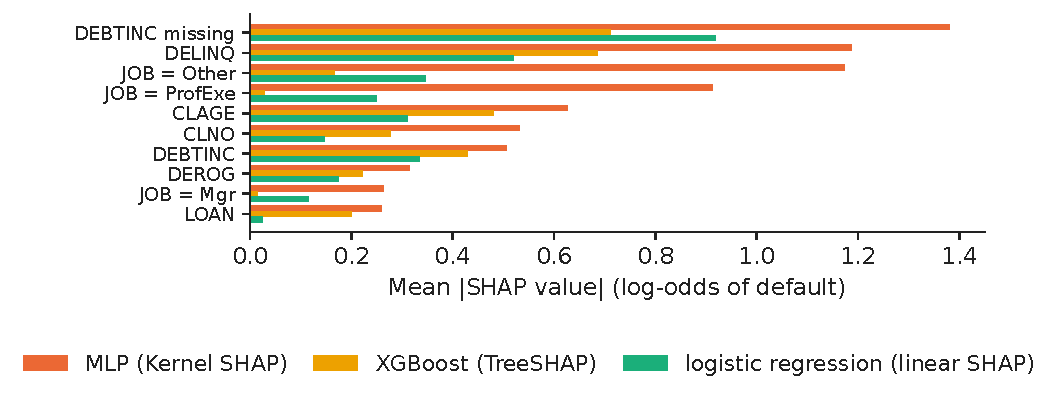
\includegraphics[width=\textwidth,height=0.292\textheight,keepaspectratio]{charts/en/shap_global.pdf}\end{center}\vspace{-3mm}
\chartsource{Source: Baesens, Roesch and Scheule (2016), HMEQ data. Data: 400 test applicants, 100 background applicants.}
\vspace{0.5mm}
\begin{itemize}\setlength{\itemsep}{0pt}
  \item Top for all three models: DEBTINC\_missing
    \begin{itemize}\setlength{\itemsep}{0pt}
      \item MLP: then DELINQ and JOB\_Other
      \item Spearman correlation of importances MLP--XGBoost 0.55, MLP--logistic 0.79.
    \end{itemize}
  \item Debt-to-income ratio (DEBTINC) missing for 21.3\,\% of loans
    \begin{itemize}\setlength{\itemsep}{0pt}
      \item Default rate 62.0\,\% when missing vs 8.6\,\% when reported.
    \end{itemize}
\end{itemize}
\par\vfill\manager{an explanation can reveal that a model scores the paperwork rather than the borrower
    \begin{itemize}\setlength{\itemsep}{0pt}
      \item Decide whether that is acceptable.
    \end{itemize}}\par\vspace{0.5mm}
\par\vfill\noindent{\scriptsize\color{FooterGray}(own computation)}\hfill\qlink{NN\_L11\_shap\_global}{Quantlets/L11/NN_L11_shap_global}\par\vspace{0.5mm}
\end{frame}

\begin{frame}{The beeswarm: direction and spread of every effect}
\small
\intuition{each dot is one applicant; colour = rank of the feature value; position = its SHAP value.}
\begin{center}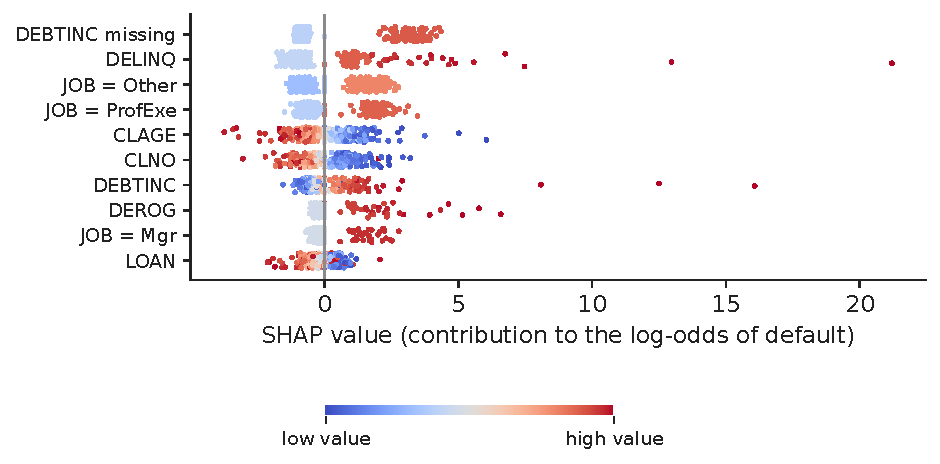
\includegraphics[width=\textwidth,height=0.500\textheight,keepaspectratio]{charts/en/shap_beeswarm.pdf}\end{center}\vspace{-3mm}
\chartsource{Source: Baesens, Roesch and Scheule (2016), HMEQ data. Data: 400 test applicants; colour = rank of the feature value.}
\vspace{0.5mm}
\begin{itemize}\setlength{\itemsep}{0pt}
  \item Delinquent credit lines (DELINQ) and derogatory reports (DEROG): high values push the risk up, as credit theory expects.
\end{itemize}
\par\vfill\noindent{\scriptsize\color{FooterGray}(own computation)}\hfill\qlink{NN\_L11\_shap\_beeswarm}{Quantlets/L11/NN_L11_shap_beeswarm}\par\vspace{0.5mm}
\end{frame}

\begin{frame}{Why was this applicant rejected? A SHAP waterfall}
\small
\intuition{from the average log-odds $\phi_0$ to this applicant's score, one feature at a time.}
\begin{center}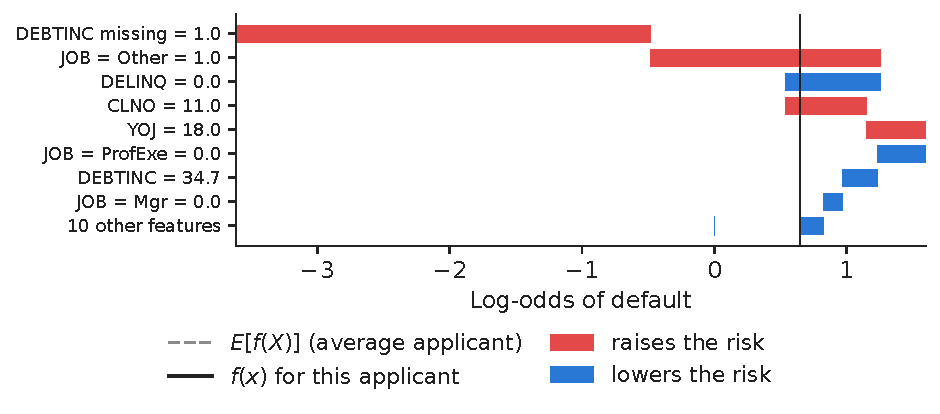
\includegraphics[width=\textwidth,height=0.475\textheight,keepaspectratio]{charts/en/shap_waterfall.pdf}\end{center}\vspace{-3mm}
\chartsource{Source: Baesens, Roesch and Scheule (2016), HMEQ data. Data: test applicant (row 2411); values in original units.}
\vspace{0.5mm}
\begin{itemize}\setlength{\itemsep}{0pt}
  \item Test applicant (row 2411): PD 65.6\,\%, log-odds 0.648 = \ensuremath{-}3.613 + 4.261
    \begin{itemize}\setlength{\itemsep}{0pt}
      \item Largest pushes: DEBTINC\_missing (\ensuremath{+}3.13), JOB\_Other (\ensuremath{+}1.74), DELINQ (\ensuremath{-}0.71).
    \end{itemize}
\end{itemize}
\par\vfill\manager{the adverse-action notice lists the top reasons in this order, in words the customer understands.}\par\vspace{0.5mm}
\par\vfill\noindent{\scriptsize\color{FooterGray}(own computation)}\hfill\qlink{NN\_L11\_shap\_waterfall}{Quantlets/L11/NN_L11_shap_waterfall}\par\vspace{0.5mm}
\end{frame}

\begin{frame}{Dependence plot: the network learned the missing-value signal}
\small
\intuition{SHAP value of DEBTINC against its value; red points are imputed at the training median.}
\begin{center}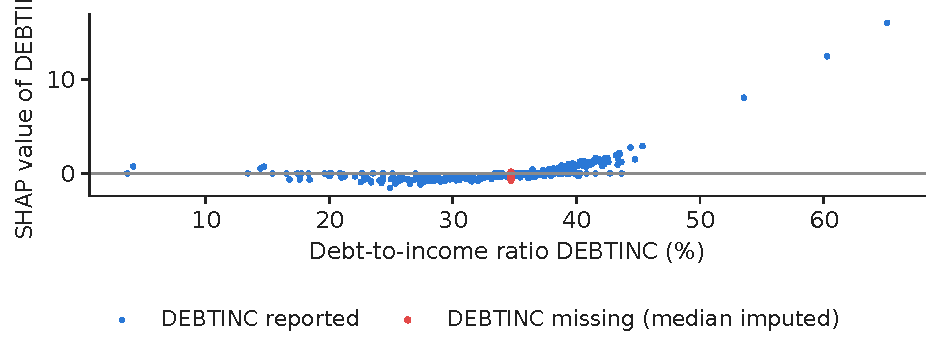
\includegraphics[width=\textwidth,height=0.376\textheight,keepaspectratio]{charts/en/shap_dependence.pdf}\end{center}\vspace{-3mm}
\chartsource{Source: Baesens, Roesch and Scheule (2016), HMEQ data. Data: 400 test applicants, MLP.}
\vspace{0.5mm}
\begin{itemize}\setlength{\itemsep}{0pt}
  \item Imputed applicants sit at one DEBTINC value
    \begin{itemize}\setlength{\itemsep}{0pt}
      \item Their risk is carried by the missing flag (mean SHAP \ensuremath{+}3.13), not by DEBTINC itself.
    \end{itemize}
\end{itemize}
\par\vfill\manager{imputation choices change explanations
    \begin{itemize}\setlength{\itemsep}{0pt}
      \item Keep a missing-value flag so that the reason can be named.
    \end{itemize}}\par\vspace{0.5mm}
\par\vfill\noindent{\scriptsize\color{FooterGray}(own computation)}\hfill\qlink{NN\_L11\_shap\_dependence}{Quantlets/L11/NN_L11_shap_dependence}\par\vspace{0.5mm}
\end{frame}


\section{LIME, counterfactuals and global effects}

\begin{frame}{LIME: a simple model that is faithful near one point}
\footnotesize
\intuition{perturb the applicant, weight the perturbations by closeness, fit a sparse linear model to the network's answers.}
\begin{columns}[T,onlytextwidth]
\begin{column}{0.56\textwidth}
\[ \xi(\vx)=\argmin_{g\in\mathcal{G}}\ \sum_{\vz}\pi_{\vx}(\vz)\big[f(\vz)-g(\vz)\big]^2+\Omega(g) \]\[ \pi_{\vx}(\vz)=\exp\!\Big(-\frac{\|\vz-\vx\|^2}{\sigma^2}\Big) \]{\footnotesize\begin{itemize}\setlength{\itemsep}{0pt}
  \item \textbf{\txtwhere}
    \begin{itemize}\setlength{\itemsep}{0pt}
      \item $\mathcal{G}$ = linear models $g(\vz)=\beta_0+\boldsymbol\beta^{\top}\vz$
      \item $\Omega$ = complexity penalty
      \item $\vz\sim\mathcal{N}(\vx,\mathbf{I})$ in standardised units
      \item Kernel width $\sigma=0.75\sqrt{d}$ = 3.18 by default.
    \end{itemize}
\end{itemize}\par}
\end{column}
\begin{column}{0.41\textwidth}
\begin{itemize}\setlength{\itemsep}{3pt}
  \item \textbf{Local slope}, not a split of the prediction: the coefficients do not add up to $f(\vx)$.
  \item \textbf{Three choices} decide the answer: neighbourhood, kernel width, number of samples.
  \item \textbf{Our applicant}: LIME's top feature is DELINQ, SHAP's is DEBTINC\_missing.
\end{itemize}
\end{column}
\end{columns}
\par\vfill\manager{LIME answers ``what moves the score near this customer?'', SHAP answers ``why is this customer far from average?''.}\par\vspace{0.5mm}
\par\vfill\noindent{\scriptsize\color{FooterGray}(Ribeiro, Singh \& Guestrin, 2016)}\hfill\tryit{notebook \S3}\par\vspace{0.5mm}
\end{frame}

\begin{frame}{LIME and SHAP for the same applicant}
\small
\intuition{LIME slope times the standardised value, next to the SHAP contribution, for the eight largest SHAP features.}
\begin{center}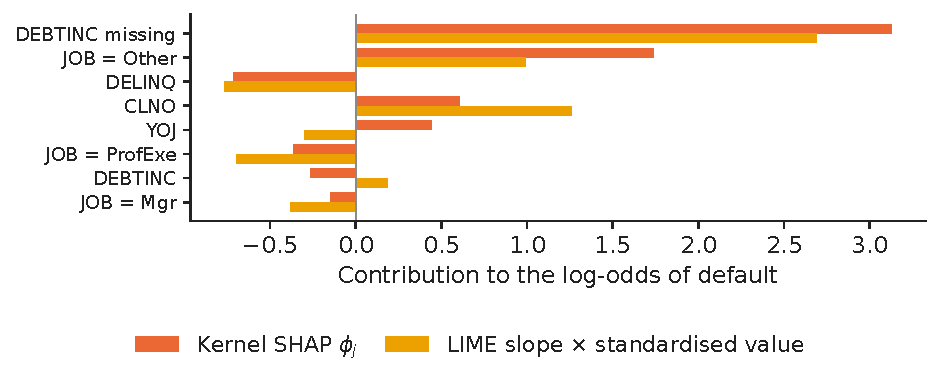
\includegraphics[width=\textwidth,height=0.500\textheight,keepaspectratio]{charts/en/lime_vs_shap.pdf}\end{center}\vspace{-3mm}
\chartsource{Source: Baesens, Roesch and Scheule (2016), HMEQ data. Data: test applicant (row 2411); LIME with 5,000 samples.}
\vspace{0.5mm}
\begin{itemize}\setlength{\itemsep}{0pt}
  \item Spearman correlation of the absolute contributions: 0.80
    \begin{itemize}\setlength{\itemsep}{0pt}
      \item A binary flag is far from its local linear approximation.
    \end{itemize}
\end{itemize}
\par\vfill\noindent{\scriptsize\color{FooterGray}(own computation)}\hfill\qlink{NN\_L11\_lime\_vs\_shap}{Quantlets/L11/NN_L11_lime_vs_shap}\par\vspace{0.5mm}
\end{frame}

\begin{frame}{LIME depends on its own settings}
\small
\intuition{left: 30 runs with different random seeds; right: the five slopes as the kernel width changes.}
\begin{center}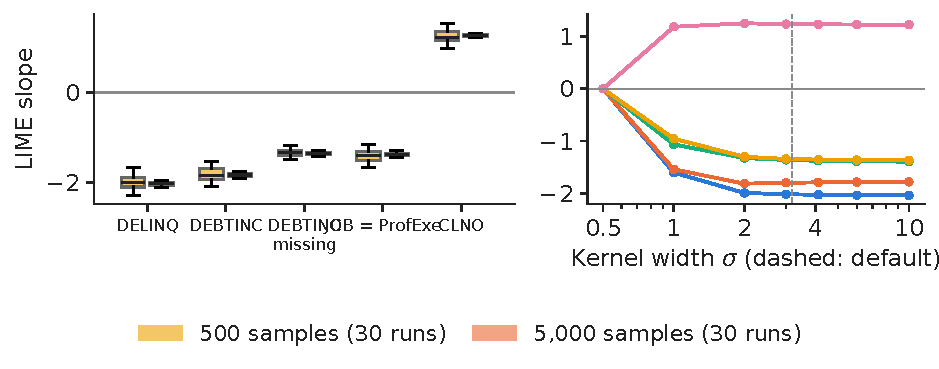
\includegraphics[width=\textwidth,height=0.321\textheight,keepaspectratio]{charts/en/lime_instability.pdf}\end{center}\vspace{-3mm}
\chartsource{Source: Baesens, Roesch and Scheule (2016), HMEQ data. Data: test applicant (row 2411); right panel: same five features, 5,000 samples.}
\vspace{0.5mm}
\begin{itemize}\setlength{\itemsep}{0pt}
  \item Same top feature: 73\,\% of runs with 500 samples, 100\,\% with 5,000
    \begin{itemize}\setlength{\itemsep}{0pt}
      \item Jaccard overlap of the top-5 sets 0.72 vs 1.00
      \item Coefficient of variation 10\,\% vs 2\,\%.
    \end{itemize}
\end{itemize}
\par\vfill\manager{fix and report the seed, sample size and kernel width of every LIME explanation that reaches a customer or an auditor.}\par\vspace{0.5mm}
\par\vfill\noindent{\scriptsize\color{FooterGray}(own computation)}\hfill\qlink{NN\_L11\_lime\_instability}{Quantlets/L11/NN_L11_lime_instability}\par\vspace{0.5mm}
\end{frame}

\begin{frame}{Counterfactual explanations: what would have to change?}
\footnotesize
\intuition{find the closest applicant, in actionable features only, whom the model would accept.}
\begin{columns}[T,onlytextwidth]
\begin{column}{0.55\textwidth}
\[ \vx'=\argmin_{\vx'}\ \lambda\,\big(f(\vx')-t\big)_+^{2}+\sum_{j\in\mathcal{A}}\frac{|x'_j-x_j|}{\mathrm{MAD}_j} \]{\footnotesize\begin{itemize}\setlength{\itemsep}{0pt}
  \item \textbf{\txtwhere}
    \begin{itemize}\setlength{\itemsep}{0pt}
      \item $t$ = target log-odds ($-0.5$, below the 0.5 PD threshold)
      \item $\mathcal{A}$ = actionable features (LOAN, DEBTINC, NINQ, DELINQ, DEROG, CLNO, MORTDUE)
      \item Median absolute deviation (MAD) scales the distance
      \item Raw values kept $\ge0$, counts rounded.
    \end{itemize}
\end{itemize}\par}
\end{column}
\begin{column}{0.42\textwidth}
{\footnotesize\renewcommand{\arraystretch}{1.05}\setlength{\tabcolsep}{4pt}
\begin{tabular}{@{}lrr@{}}\toprule
Feature & now & needed \\ \midrule
MORTDUE & 69\,115.0 & 57\,456.5 \\
DEBTINC & 34.7 & 33.4 \\
LOAN & 14\,500.0 & 15\,700.0 \\
\bottomrule\end{tabular}}\begin{itemize}\setlength{\itemsep}{1pt}
  \item PD 65.6\,\% $\to$ 39.2\,\% after these changes.
  \item Documentary counterfactual: reporting DEBTINC (at the median 34.7) gives PD 5.1\,\%.
\end{itemize}
\end{column}
\end{columns}
\par\vfill\manager{``bring the missing income document'' is a better answer to the customer than any list of SHAP values.}\par\vspace{0.5mm}
\par\vfill\noindent{\scriptsize\color{FooterGray}(Wachter, Mittelstadt \& Russell, 2017)}\hfill\tryit{notebook \S4}\par\vspace{0.5mm}
\end{frame}

\begin{frame}{Global effects: partial dependence and ICE}
\small
\intuition{the PDP averages the prediction over the data while one feature is set to a grid value; ICE keeps one curve per observation.}
\vspace{-1mm}\[ \mathrm{PD}_j(z)=\frac1n\sum_{i=1}^{n}f(z,\vx_{i,-j}),\qquad \mathrm{ICE}_{i,j}(z)=f(z,\vx_{i,-j}) \]\vspace{-2mm}
\begin{center}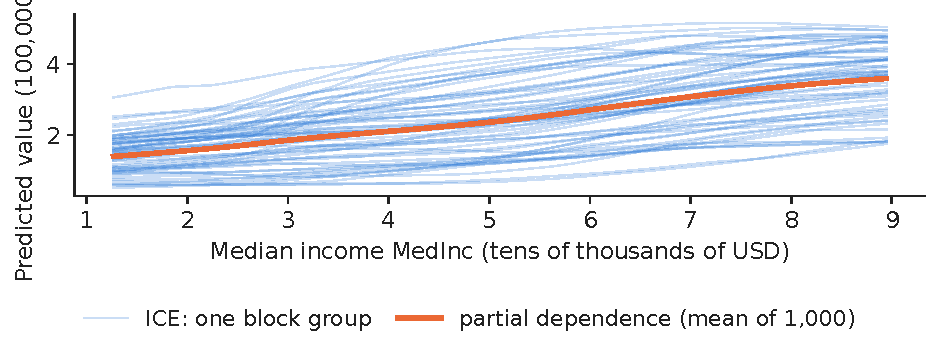
\includegraphics[width=\textwidth,height=0.350\textheight,keepaspectratio]{charts/en/pdp_ice.pdf}\end{center}\vspace{-3mm}
\chartsource{Source: StatLib, California housing, 1990 census (Pace and Barry, 1997). Data: MLP; 60 test block groups (ICE), 1,000 for the PDP.}
\vspace{0.5mm}
\begin{itemize}\setlength{\itemsep}{0pt}
  \item California housing MLP (test $R^2$ 0.819, linear 0.620): the predicted value rises from 1.40 to 3.60 (100,000 USD) over the income grid
    \begin{itemize}\setlength{\itemsep}{0pt}
      \item Spread of the ICE curves at the top 0.95.
    \end{itemize}
\end{itemize}
\par\vfill\noindent{\scriptsize\color{FooterGray}(Friedman, 2001; Goldstein et al., 2015)}\hfill\qlink{NN\_L11\_pdp\_ice}{Quantlets/L11/NN_L11_pdp_ice}\par\vspace{0.5mm}
\end{frame}


\section{Gradient methods for neural networks}

\begin{frame}{The fraud case: a network trained on day 1, explained on day 2}
\footnotesize
\intuition{gradients are free for a network: one backward pass gives the sensitivity of the fraud score to every input.}
\begin{columns}[T,onlytextwidth]
\begin{column}{0.55\textwidth}
\[ \mathrm{saliency}_j(\vx)=\Big|\frac{\partial f(\vx)}{\partial x_j}\Big|,\qquad \mathrm{G\!\times\!I}_j(\vx)=(x_j-x'_j)\,\frac{\partial f(\vx)}{\partial x_j} \]{\footnotesize\begin{itemize}\setlength{\itemsep}{0pt}
  \item \textbf{\txtwhere}
    \begin{itemize}\setlength{\itemsep}{0pt}
      \item $f$ = fraud log-odds of an MLP on V1--V28 and log amount
      \item $\vx'$ = baseline = mean legitimate transaction of day 1
      \item Class weight $\sqrt{\text{imbalance}}$, early stopping on weighted validation PR-AUC.
    \end{itemize}
\end{itemize}\par}
\end{column}
\begin{column}{0.42\textwidth}
\begin{itemize}\setlength{\itemsep}{3pt}
  \item \textbf{Test, day 2} (full-data weights): MLP PR-AUC 0.815, logistic 0.742
    \begin{itemize}\setlength{\itemsep}{0pt}
      \item AUC 0.961 vs 0.964.
    \end{itemize}
  \item \textbf{Saturation}: in a flat region of $f$ the gradient is near zero even for a decisive feature.
  \item \textbf{ReLU networks}: the gradient is piecewise constant, so saliency jumps between linear regions.
\end{itemize}
\end{column}
\end{columns}
\par\vfill\manager{a fraud analyst gets a ranked list of the inputs that drove the alert, in milliseconds per transaction.}\par\vspace{0.5mm}
\par\vfill\noindent{\scriptsize\color{FooterGray}(Simonyan, Vedaldi \& Zisserman, 2014; Dal Pozzolo et al., 2015)}\hfill\tryit{notebook \S5}\par\vspace{0.5mm}
\end{frame}

\begin{frame}{Integrated gradients: attributions that add up}
\footnotesize
\intuition{integrate the gradient along the straight path from a baseline to the input; the attributions sum to $f(\vx)-f(\vx')$.}
\begin{columns}[T,onlytextwidth]
\begin{column}{0.6\textwidth}
\[ \mathrm{IG}_j(\vx)=(x_j-x'_j)\int_0^1\frac{\partial f\big(\vx'+\alpha(\vx-\vx')\big)}{\partial x_j}\,d\alpha \]\[ \approx(x_j-x'_j)\frac1m\sum_{k=1}^{m}\frac{\partial f\big(\vx'+\tfrac{k-1/2}{m}(\vx-\vx')\big)}{\partial x_j} \]{\footnotesize\begin{itemize}\setlength{\itemsep}{0pt}
  \item \textbf{\txtwhere}
    \begin{itemize}\setlength{\itemsep}{0pt}
      \item $m$ = Riemann steps (midpoint rule, 64 here)
      \item Completeness $\sum_j\mathrm{IG}_j=f(\vx)-f(\vx')$ follows from the fundamental theorem of calculus for paths.
    \end{itemize}
\end{itemize}\par}
\end{column}
\begin{column}{0.37\textwidth}
\begin{itemize}\setlength{\itemsep}{3pt}
  \item \textbf{Axioms} (Sundararajan et al., 2017)
    \begin{itemize}\setlength{\itemsep}{0pt}
      \item Completeness; sensitivity: a feature that changes $f$ gets non-zero credit
      \item Implementation invariance: equal functions, equal attributions
    \end{itemize}
  \item \textbf{Link to Shapley}: IG is the Aumann-Shapley value of the continuous game along the path.
  \item \textbf{Baseline matters}: ``mean legitimate transaction'' answers ``why is this not a normal payment?''.
\end{itemize}
\end{column}
\end{columns}
\par\vfill\manager{write the baseline into the model documentation: a different baseline is a different question.}\par\vspace{0.5mm}
\par\vfill\noindent{\scriptsize\color{FooterGray}(Sundararajan, Taly \& Yan, 2017)}\hfill\tryit{notebook \S5}\par\vspace{0.5mm}
\end{frame}

\begin{frame}{Completeness holds once the integral is computed accurately}
\small
\intuition{median of $|\sum_j\mathrm{IG}_j-(f(\vx)-f(\vx'))|/|f(\vx)-f(\vx')|$ over the frauds of day 2.}
\begin{center}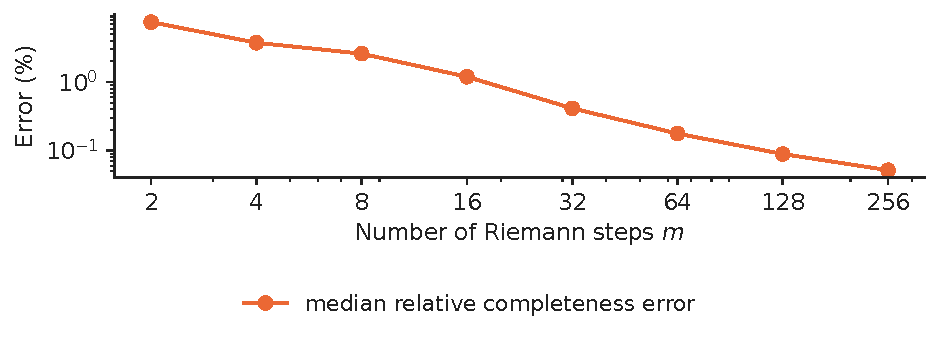
\includegraphics[width=\textwidth,height=0.500\textheight,keepaspectratio]{charts/en/ig_completeness.pdf}\end{center}\vspace{-3mm}
\chartsource{Source: ULB Machine Learning Group and Worldline, credit-card transactions (OpenML 1597). Data: 211 frauds of day 2; baseline = mean legitimate transaction of day 1.}
\vspace{0.5mm}
\begin{itemize}\setlength{\itemsep}{0pt}
  \item 3.7\,\% error with 4 steps, 0.18\,\% with 64, over 211 frauds
    \begin{itemize}\setlength{\itemsep}{0pt}
      \item The error falls roughly as $1/m^{2}$, as for the midpoint rule.
    \end{itemize}
\end{itemize}
\par\vfill\noindent{\scriptsize\color{FooterGray}(own computation)}\hfill\qlink{NN\_L11\_ig\_completeness}{Quantlets/L11/NN_L11_ig_completeness}\par\vspace{0.5mm}
\end{frame}

\begin{frame}{SmoothGrad and concept-level explanations}
\footnotesize
\intuition{average gradients over noisy copies of the input to remove ReLU jitter; or ask whether a human concept moves the output.}
\begin{columns}[T,onlytextwidth]
\begin{column}{0.58\textwidth}
\[ \mathrm{SG}_j(\vx)=\frac1n\sum_{k=1}^{n}\frac{\partial f(\vx+\boldsymbol\varepsilon_k)}{\partial x_j},\quad \boldsymbol\varepsilon_k\sim\mathcal{N}(\mathbf 0,s^{2}\mathbf I) \]\[ S_{C}(\vx)=\nabla h(\vx)^{\top}\mathbf{v}_C \]{\footnotesize\begin{itemize}\setlength{\itemsep}{0pt}
  \item \textbf{\txtwhere}
    \begin{itemize}\setlength{\itemsep}{0pt}
      \item $n=50$, $s=0.15$ standard deviations
      \item Testing with concept activation vectors (TCAV): $\mathbf{v}_C$ = normal of a linear classifier separating examples of concept $C$ in a hidden layer $h$
      \item The TCAV score is the share of inputs with $S_C>0$.
    \end{itemize}
\end{itemize}\par}
\end{column}
\begin{column}{0.39\textwidth}
\begin{itemize}\setlength{\itemsep}{3pt}
  \item \textbf{SmoothGrad} sharpens image saliency maps and stabilises tabular gradients (next section).
  \item \textbf{TCAV} speaks the language of the business: ``night-time transaction'', ``new merchant'' --- if such concepts are labelled.
  \item \textbf{Our data}: V1--V28 are anonymised components, so concept tests are not possible here.
\end{itemize}
\end{column}
\end{columns}
\par\vfill\manager{concept explanations need concepts labelled when the data are collected.}\par\vspace{0.5mm}
\par\vfill\noindent{\scriptsize\color{FooterGray}(Smilkov et al., 2017; Kim et al., 2018)}\par\vspace{0.5mm}
\end{frame}

\begin{frame}{One fraud, four explanations}
\small
\intuition{signed attributions of one day-2 fraud (median fraud score), as shares of the total absolute attribution.}
\begin{center}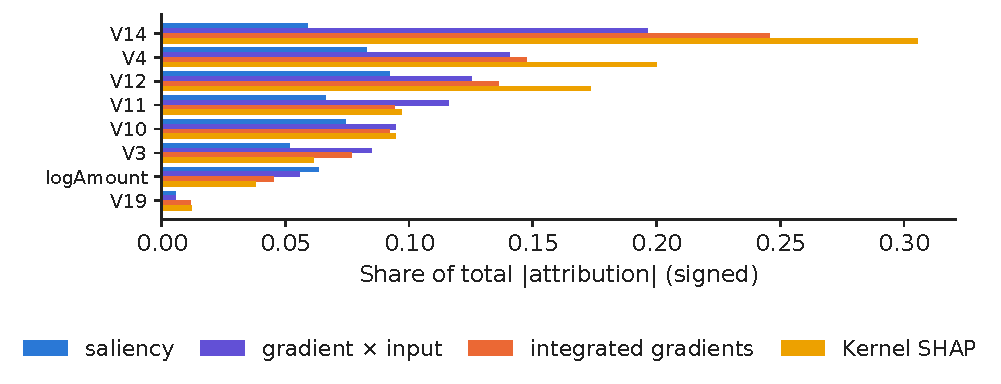
\includegraphics[width=\textwidth,height=0.485\textheight,keepaspectratio]{charts/en/fraud_local.pdf}\end{center}\vspace{-3mm}
\chartsource{Source: ULB Machine Learning Group and Worldline, credit-card transactions (OpenML 1597). Data: one fraud of day 2 (median fraud score).}
\vspace{0.5mm}
\begin{itemize}\setlength{\itemsep}{0pt}
  \item Top feature: Kernel SHAP V14, integrated gradients V14, saliency V12
    \begin{itemize}\setlength{\itemsep}{0pt}
      \item Fraud score 99.9\,\%: saliency is blind to the size of the deviation from the baseline.
    \end{itemize}
\end{itemize}
\par\vfill\noindent{\scriptsize\color{FooterGray}(own computation)}\hfill\qlink{NN\_L11\_fraud\_local}{Quantlets/L11/NN_L11_fraud_local}\par\vspace{0.5mm}
\end{frame}


\section{Do explanations agree, are they faithful, are they stable?}

\begin{frame}{Agreement between methods: high but not perfect}
\small
\intuition{Spearman correlation of the global importances (mean $|$attribution$|$) of seven methods on the same frauds.}
\begin{center}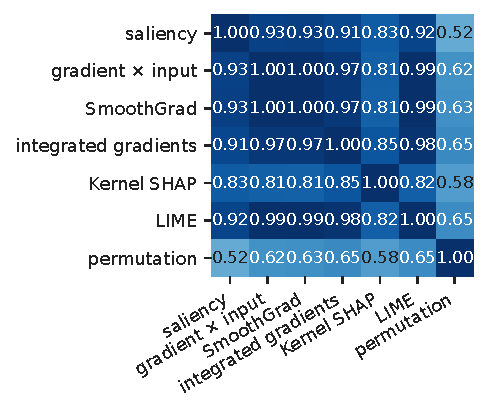
\includegraphics[width=\textwidth,height=0.370\textheight,keepaspectratio]{charts/en/method_agreement.pdf}\end{center}\vspace{-3mm}
\chartsource{Source: ULB Machine Learning Group and Worldline, credit-card transactions (OpenML 1597). Data: Spearman correlation of global importances; 211 frauds of day 2.}
\vspace{0.5mm}
\begin{itemize}\setlength{\itemsep}{0pt}
  \item IG--SHAP 0.85, saliency--SHAP 0.83, LIME--SHAP 0.82, permutation--SHAP 0.58
    \begin{itemize}\setlength{\itemsep}{0pt}
      \item All methods put V12 first.
    \end{itemize}
\end{itemize}
\par\vfill\manager{disagreement is information: permutation importance measures what the model needs, attributions what it uses.}\par\vspace{0.5mm}
\par\vfill\noindent{\scriptsize\color{FooterGray}(Breiman, 2001; own computation)}\hfill\qlink{NN\_L11\_method\_agreement}{Quantlets/L11/NN_L11_method_agreement}\par\vspace{0.5mm}
\end{frame}

\begin{frame}{Faithfulness: remove what the explanation says matters}
\small
\intuition{reset the top-$k$ features of each fraud to the baseline; a faithful explanation makes the score fall fast.}
\vspace{-1mm}\[ \mathrm{AOPC}=\frac{1}{K}\sum_{k=1}^{K}\big[f(\vx)-f(\vx^{(k)})\big] \]\vspace{-2mm}
\begin{center}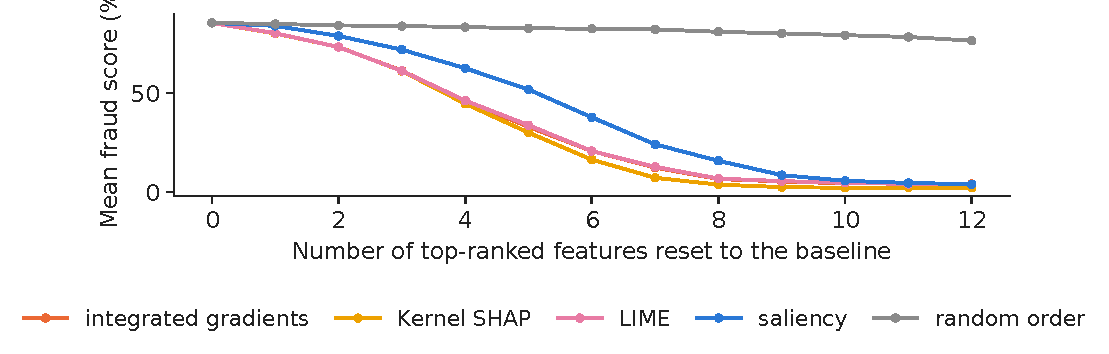
\includegraphics[width=\textwidth,height=0.379\textheight,keepaspectratio]{charts/en/deletion_curve.pdf}\end{center}\vspace{-3mm}
\chartsource{Source: ULB Machine Learning Group and Worldline, credit-card transactions (OpenML 1597). Data: 211 frauds of day 2.}
\vspace{0.5mm}
\begin{itemize}\setlength{\itemsep}{0pt}
  \item Area over the perturbation curve (AOPC) in points of fraud score: IG 56.2, SHAP 58.4, LIME 56.1, saliency 48.0, random order 3.9.
\end{itemize}
\par\vfill\noindent{\scriptsize\color{FooterGray}(Samek et al., 2017)}\hfill\qlink{NN\_L11\_deletion\_curve}{Quantlets/L11/NN_L11_deletion_curve}\par\vspace{0.5mm}
\end{frame}

\begin{frame}{Local robustness: small input change, small explanation change?}
\small
\intuition{relative change of the attribution vector per unit of a small perturbation (Lipschitz-type ratio).}
\vspace{-1mm}\[ \hat L(\vx)=\frac{\|\mathbf a(\vx+\boldsymbol\varepsilon)-\mathbf a(\vx)\|/\|\mathbf a(\vx)\|}{\|\boldsymbol\varepsilon\|},\quad \boldsymbol\varepsilon\sim\mathcal N(\mathbf 0,0.05^{2}\mathbf I) \]\vspace{-2mm}
\begin{center}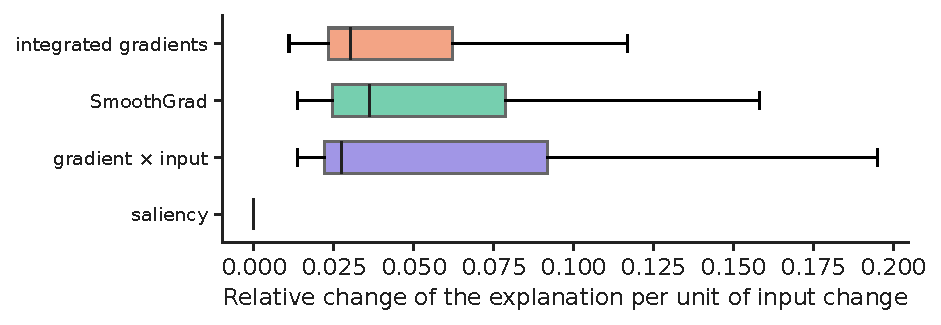
\includegraphics[width=\textwidth,height=0.385\textheight,keepaspectratio]{charts/en/local_robustness.pdf}\end{center}\vspace{-3mm}
\chartsource{Source: ULB Machine Learning Group and Worldline, credit-card transactions (OpenML 1597). Data: 60 frauds of day 2 x 10 perturbations (sigma = 0.05 standard deviations).}
\vspace{0.5mm}
\begin{itemize}\setlength{\itemsep}{0pt}
  \item Medians: saliency 0.000, gradient $\times$ input 0.028, IG 0.030, SmoothGrad 0.036
    \begin{itemize}\setlength{\itemsep}{0pt}
      \item Within a linear region of a ReLU network the gradient does not move.
    \end{itemize}
\end{itemize}
\par\vfill\noindent{\scriptsize\color{FooterGray}(Alvarez-Melis \& Jaakkola, 2018)}\hfill\qlink{NN\_L11\_local\_robustness}{Quantlets/L11/NN_L11_local_robustness}\par\vspace{0.5mm}
\end{frame}

\begin{frame}{The Rashomon effect: same accuracy, different explanations}
\small
\intuition{rank of each feature by mean $|$SHAP$|$ for 10 retrained networks and 10 boosted ensembles (different seeds only).}
\begin{center}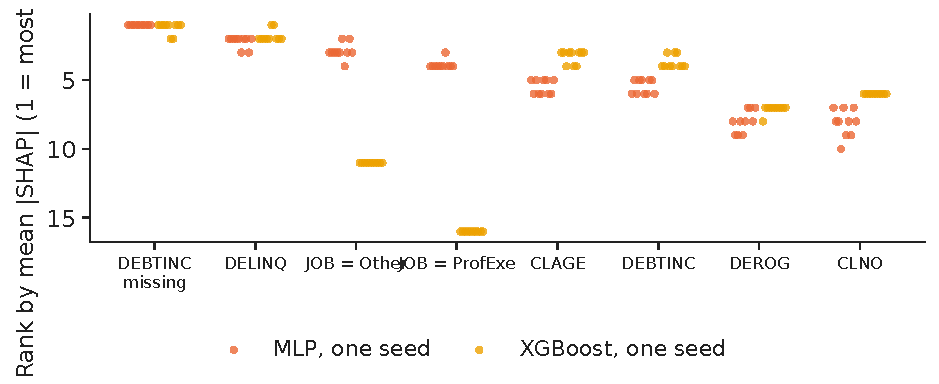
\includegraphics[width=\textwidth,height=0.420\textheight,keepaspectratio]{charts/en/seed_stability.pdf}\end{center}\vspace{-3mm}
\chartsource{Source: Baesens, Roesch and Scheule (2016), HMEQ data. Data: 10 training seeds; 200 test applicants.}
\vspace{0.5mm}
\begin{itemize}\setlength{\itemsep}{0pt}
  \item MLP test AUC between 0.929 and 0.941
    \begin{itemize}\setlength{\itemsep}{0pt}
      \item Mean pairwise Kendall $\tau$ (rank agreement of importances, 1 = identical order): MLP 0.83, XGBoost 0.97
      \item Same top feature for one applicant in 78\,\% (MLP) and 83\,\% (XGBoost) of seed pairs.
    \end{itemize}
\end{itemize}
\par\vfill\noindent{\scriptsize\color{FooterGray}(own computation)}\hfill\qlink{NN\_L11\_seed\_stability}{Quantlets/L11/NN_L11_seed_stability}\par\vspace{0.5mm}
\end{frame}

\begin{frame}{Explanations over time: day 1 against day 2}
\small
\intuition{share of the total $|$IG$|$ by feature, for held-out frauds of the training day and for the frauds of the next day.}
\begin{center}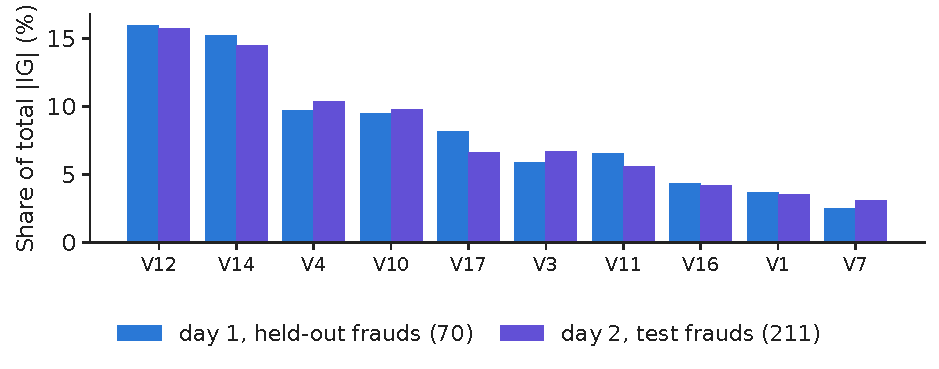
\includegraphics[width=\textwidth,height=0.286\textheight,keepaspectratio]{charts/en/time_shift.pdf}\end{center}\vspace{-3mm}
\chartsource{Source: ULB Machine Learning Group and Worldline, credit-card transactions (OpenML 1597). Data: model trained on day 1; integrated gradients.}
\vspace{0.5mm}
\begin{itemize}\setlength{\itemsep}{0pt}
  \item Spearman 0.98, Jensen-Shannon (JS) divergence (built on the Kullback-Leibler (KL) divergence) 0.003, 4 of the top 5 shared
    \begin{itemize}\setlength{\itemsep}{0pt}
      \item One day later the explanation is stable here.
    \end{itemize}
\end{itemize}
\par\vfill\manager{monitor the distribution of attributions monthly, next to the score distribution
    \begin{itemize}\setlength{\itemsep}{0pt}
      \item A drift in reasons can precede a drift in accuracy.
    \end{itemize}}\par\vspace{0.5mm}
\par\vfill\noindent{\scriptsize\color{FooterGray}(own computation)}\hfill\qlink{NN\_L11\_time\_shift}{Quantlets/L11/NN_L11_time_shift}\par\vspace{0.5mm}
\end{frame}

\begin{frame}{Stability scorecard of this lecture}
\small
{\footnotesize\renewcommand{\arraystretch}{1.05}\setlength{\tabcolsep}{4pt}
\begin{tabular}{@{}p{0.3\textwidth}p{0.32\textwidth}p{0.3\textwidth}@{}}\toprule
Source of change & Measure & Result \\ \midrule
Explainer randomness (LIME) & same top feature over 30 runs & 73\,\% (500), 100\,\% (5,000 samples) \\
Training seed (Rashomon) & Kendall $\tau$ of global importances & MLP 0.83, XGBoost 0.97 \\
Training seed, one applicant & same top feature & MLP 78\,\%, XGBoost 83\,\% \\
Method & Spearman of importances & 0.52 -- 1.00 \\
Input noise & median relative change & IG 0.030, SmoothGrad 0.036 \\
Time (day 1 $\to$ day 2) & Spearman, JS divergence & 0.98; 0.003 \\
\bottomrule\end{tabular}}
\par\vfill\manager{report every explanation with its stability: which seed, which sample, which period, and how much it moves.}\par\vspace{0.5mm}
\par\vfill\noindent{\scriptsize\color{FooterGray}(own computation)}\par\vspace{0.5mm}
\end{frame}


\section{Explainability in model governance}

\begin{frame}{An explainability audit checklist}
\small
\begin{columns}[T,onlytextwidth]
\begin{column}{0.49\textwidth}
\begin{itemize}\setlength{\itemsep}{4pt}
  \item \textbf{Purpose}: who reads the explanation (customer, analyst, validator, regulator) and what decision it supports.
  \item \textbf{Settings}: background sample, baseline, seed, number of samples, kernel width --- versioned with the model.
  \item \textbf{Checks}: additivity/completeness, faithfulness (deletion), stability (seeds, time), agreement of two methods.
\end{itemize}
\end{column}
\begin{column}{0.49\textwidth}
\begin{itemize}\setlength{\itemsep}{4pt}
  \item \textbf{Fairness}: attributions of protected attributes and of their proxies (age, sex, postcode)
    \begin{itemize}\setlength{\itemsep}{0pt}
      \item An explanation shows use, not causation.
    \end{itemize}
  \item \textbf{Customer output}: few reasons, actionable counterfactuals, no raw component names (V14 means nothing to a customer).
  \item \textbf{Alternative}: if an interpretable model is almost as accurate (here logistic AUC 0.909 vs MLP 0.935), consider using it.
\end{itemize}
\end{column}
\end{columns}
\par\vfill\manager{the validation report should contain the explanations and their stability tests, not only the accuracy.}\par\vspace{0.5mm}
\par\vfill\noindent{\scriptsize\color{FooterGray}(SR 11-7; Rudin, 2019)}\par\vspace{0.5mm}
\end{frame}

\section*{Wrap-up}

\begin{frame}{Quiz 1: adding up SHAP values}
\small
\begin{itemize}
  \item For our applicant the base value is \ensuremath{-}3.613 and the SHAP values sum to 4.261.
    \begin{itemize}\setlength{\itemsep}{0pt}
      \item What is the model's log-odds of default, and why can you be sure?
    \end{itemize}
\end{itemize}
\vspace{2mm}
\begin{exampleblock}{Answer}
\begin{itemize}
  \item 0.648: by the efficiency axiom $f(\vx)=\phi_0+\sum_j\phi_j$
    \begin{itemize}\setlength{\itemsep}{0pt}
      \item The PD is $\sigma$(0.648) = 65.6\,\%.
    \end{itemize}
\end{itemize}
\end{exampleblock}
\end{frame}

\begin{frame}{Quiz 2: an unstable LIME}
\small
\begin{itemize}
  \item Two analysts explain the same rejected applicant with LIME and report different top reasons.
    \begin{itemize}\setlength{\itemsep}{0pt}
      \item Is the model inconsistent?
    \end{itemize}
\end{itemize}
\vspace{2mm}
\begin{exampleblock}{Answer}
\begin{itemize}
  \item Not necessarily: LIME samples perturbations
    \begin{itemize}\setlength{\itemsep}{0pt}
      \item With 500 samples the top feature matched in 73\,\% of our runs
      \item Fix the seed, raise the samples, check against SHAP.
    \end{itemize}
\end{itemize}
\end{exampleblock}
\end{frame}

\begin{frame}{Quiz 3: choosing an IG baseline}
\small
\begin{itemize}
  \item A colleague uses the all-zero vector as the integrated-gradients baseline for standardised fraud features.
    \begin{itemize}\setlength{\itemsep}{0pt}
      \item What question does that explanation answer?
    \end{itemize}
\end{itemize}
\vspace{2mm}
\begin{exampleblock}{Answer}
\begin{itemize}
  \item ``Why does this transaction differ from the average transaction (frauds included)?''
    \begin{itemize}\setlength{\itemsep}{0pt}
      \item Our baseline, the mean legitimate transaction, asks why it is not a normal payment.
    \end{itemize}
\end{itemize}
\end{exampleblock}
\end{frame}

\begin{frame}{Wrap-up}
\small
\begin{itemize}\setlength{\itemsep}{4pt}
  \item \textbf{SHAP}: Shapley values with an exact additivity check
    \begin{itemize}\setlength{\itemsep}{0pt}
      \item The missing debt-to-income ratio drives the credit network.
    \end{itemize}
  \item \textbf{LIME}: a local slope that depends on seed, sample size and kernel width
    \begin{itemize}\setlength{\itemsep}{0pt}
      \item Useful, but report its settings.
    \end{itemize}
  \item \textbf{Gradients}: integrated gradients satisfy completeness (0.18\,\% error at 64 steps) and are as faithful as SHAP at a fraction of the cost.
  \item \textbf{Stability}: retraining with another seed reorders features (Kendall $\tau$ 0.83 for the MLP)
    \begin{itemize}\setlength{\itemsep}{0pt}
      \item Explanations must be tested like models.
    \end{itemize}
  \item \textbf{Next}: Lecture 12, large language models, where explanations become text.
\end{itemize}
\end{frame}

\begin{frame}{Research from our group: XAI in fraud and energy markets}
\footnotesize
\begin{itemize}\setlength{\itemsep}{4pt}
  \item \textbf{SHAP stability in graph-augmented fraud detection}: on the IEEE-CIS fraud data, SHAP contributions of an XGBoost model with graph neural network (GNN) embeddings are compared under random and forward-time validation, with a Gaussian control of the same dimension and covariance
    \begin{itemize}\setlength{\itemsep}{0pt}
      \item Whether the graph model looks more stable depends on how the change is measured, a careful protocol for explanation stability (Diaconu \& Pele, 2026, submitted to Expert Systems with Applications; code: QuantLet GNN\_XAI\_Stability).
    \end{itemize}
  \item \textbf{Explainable early warning of electricity price spikes} in Romania (Andrei, Pele, Cramer, Amza \& Diaconu, 2026, Proceedings of the International Conference on Business Excellence (PICBE)) and \textbf{SHAP-driven anomaly detection} of electricity prices (Andrei \& Pele, 2025, Preprints).
  \item \textbf{Multi-horizon explainability} of price forecasts: which drivers matter at which horizon in Romania's liberalised market (Andrei, Pele \& Cramer, 2026, PICBE).
\end{itemize}\par\vspace{1mm}{\scriptsize \begin{itemize}
  \item Findings as stated in the papers; numbers on the other slides come from our own data.
\end{itemize}}
\par\vfill\noindent{\scriptsize\color{FooterGray}(Bucharest University of Economic Studies (ASE); Romanian Academy, Institute for Economic Forecasting (IPE))}\par\vspace{0.5mm}
\end{frame}

\begin{frame}{Want to learn more?}
\small
\begin{columns}[T,onlytextwidth]
\begin{column}{0.5\textwidth}
\begin{itemize}\setlength{\itemsep}{4pt}
  \item \textbf{C.\ Molnar, Interpretable Machine Learning}, free online: \href{https://christophm.github.io/interpretable-ml-book/}{christophm.github.io/interpretable-ml-book}.
  \item \textbf{SHAP library} and examples: \href{https://shap.readthedocs.io}{shap.readthedocs.io}.
  \item \textbf{Rudin (2019)}: the case for interpretable models in high-stakes decisions.
\end{itemize}
\end{column}
\begin{column}{0.47\textwidth}
\begin{itemize}\setlength{\itemsep}{4pt}
  \item \textbf{This course}: code, data, notebooks --- \href{https://github.com/danpele/NEURAL_BIZ}{github.com/danpele/NEURAL\_BIZ}.
  \item \textbf{Experiment yourself}: notebooks/L11\_notebook.ipynb
    \begin{itemize}\setlength{\itemsep}{0pt}
      \item The seminar explains a German credit model, with a fairness check.
    \end{itemize}
  \item \textbf{Replication of our stability study}: \href{https://github.com/QuantLet/GNN_XAI_Stability}{github.com/QuantLet/GNN\_XAI\_Stability}.
\end{itemize}
\end{column}
\end{columns}
\end{frame}

\begin{frame}{References (1/3)}
\scriptsize
\begin{itemize}\setlength{\itemsep}{0pt}\scriptsize
\item Alvarez-Melis, D.\ \& Jaakkola, T.\,S.\ (2018). On the robustness of interpretability methods. ICML Workshop on Human Interpretability in Machine Learning. \href{https://arxiv.org/abs/1806.08049}{arXiv:1806.08049}
\item Andrei, A.-V.\ \& Pele, D.\,T.\ (2025). Explainable AI for electricity price anomaly detection: A SHAP-driven approach in Romania's energy market. \textit{Preprints}. \href{https://doi.org/10.20944/preprints202508.0410.v1}{doi:10.20944/preprints202508.0410.v1}
\item Andrei, A.-V., Pele, D.-T.\ \& Cramer, A.-A.\ (2026). Multi-horizon explainability in energy price forecasting: Disentangling market dynamics and renewable intermittency in Romania's liberalized electricity market. \textit{Proceedings of the International Conference on Business Excellence}, 20(1), 104--117. \href{https://doi.org/10.2478/picbe-2026-0014}{doi:10.2478/picbe-2026-0014}
\item Andrei, A.-V., Pele, D.-T., Cramer, A.-A., Amza, A.\ \& Diaconu, D.\ (2026). Explainable AI-based early warning system for electricity price spikes: Evidence from the Romanian market. \textit{Proceedings of the International Conference on Business Excellence}, 20(1), 4820--4836. \href{https://doi.org/10.2478/picbe-2026-0352}{doi:10.2478/picbe-2026-0352}
\item Baesens, B., Roesch, D.\ \& Scheule, H.\ (2016). \textit{Credit Risk Analytics: Measurement Techniques, Applications, and Examples in SAS}. Wiley.
\item Breiman, L.\ (2001). Random forests. \textit{Machine Learning}, 45, 5--32. \href{https://doi.org/10.1023/A:1010933404324}{doi:10.1023/A:1010933404324}
\item Dal Pozzolo, A., Caelen, O., Johnson, R.\,A.\ \& Bontempi, G.\ (2015). Calibrating probability with undersampling for unbalanced classification. IEEE SSCI, 159--166. \href{https://doi.org/10.1109/SSCI.2015.33}{doi:10.1109/SSCI.2015.33}
\item Diaconu, D.\ \& Pele, D.\,T.\ (2026). SHAP stability across random and forward-time validation in graph-augmented fraud detection. Submitted to \textit{Expert Systems with Applications}. Code: \href{https://github.com/QuantLet/GNN_XAI_Stability}{github.com/QuantLet/GNN\_XAI\_Stability}
\end{itemize}
\end{frame}

\begin{frame}{References (2/3)}
\scriptsize
\begin{itemize}\setlength{\itemsep}{0pt}\scriptsize
\item Friedman, J.\,H.\ (2001). Greedy function approximation: A gradient boosting machine. \textit{Annals of Statistics}, 29(5), 1189--1232. \href{https://doi.org/10.1214/aos/1013203451}{doi:10.1214/aos/1013203451}
\item Goldstein, A., Kapelner, A., Bleich, J.\ \& Pitkin, E.\ (2015). Peeking inside the black box: Visualizing statistical learning with plots of individual conditional expectation. \textit{Journal of Computational and Graphical Statistics}, 24(1), 44--65. \href{https://doi.org/10.1080/10618600.2014.907095}{doi:10.1080/10618600.2014.907095}
\item Kim, B.\ et al.\ (2018). Interpretability beyond feature attribution: Quantitative testing with concept activation vectors (TCAV). ICML. \href{https://arxiv.org/abs/1711.11279}{arXiv:1711.11279}
\item Lundberg, S.\,M.\ \& Lee, S.-I.\ (2017). A unified approach to interpreting model predictions. \textit{Advances in Neural Information Processing Systems}, 30. \href{https://arxiv.org/abs/1705.07874}{arXiv:1705.07874}
\item Lundberg, S.\,M.\ et al.\ (2020). From local explanations to global understanding with explainable AI for trees. \textit{Nature Machine Intelligence}, 2, 56--67. \href{https://doi.org/10.1038/s42256-019-0138-9}{doi:10.1038/s42256-019-0138-9}
\item Ribeiro, M.\,T., Singh, S.\ \& Guestrin, C.\ (2016). ``Why should I trust you?'' Explaining the predictions of any classifier. KDD, 1135--1144. \href{https://doi.org/10.1145/2939672.2939778}{doi:10.1145/2939672.2939778}
\item Rudin, C.\ (2019). Stop explaining black box machine learning models for high stakes decisions and use interpretable models instead. \textit{Nature Machine Intelligence}, 1, 206--215. \href{https://doi.org/10.1038/s42256-019-0048-x}{doi:10.1038/s42256-019-0048-x}
\item Samek, W., Binder, A., Montavon, G., Lapuschkin, S.\ \& Müller, K.-R.\ (2017). Evaluating the visualization of what a deep neural network has learned. \textit{IEEE Transactions on Neural Networks and Learning Systems}, 28(11), 2660--2673. \href{https://doi.org/10.1109/TNNLS.2016.2599820}{doi:10.1109/TNNLS.2016.2599820}
\end{itemize}
\end{frame}

\begin{frame}{References (3/3)}
\scriptsize
\begin{itemize}\setlength{\itemsep}{0pt}\scriptsize
\item Shapley, L.\,S.\ (1953). A value for n-person games. In \textit{Contributions to the Theory of Games II}, 307--317. Princeton University Press.
\item Simonyan, K., Vedaldi, A.\ \& Zisserman, A.\ (2014). Deep inside convolutional networks: Visualising image classification models and saliency maps. ICLR Workshop. \href{https://arxiv.org/abs/1312.6034}{arXiv:1312.6034}
\item Smilkov, D., Thorat, N., Kim, B., Viégas, F.\ \& Wattenberg, M.\ (2017). SmoothGrad: Removing noise by adding noise. \href{https://arxiv.org/abs/1706.03825}{arXiv:1706.03825}
\item Sundararajan, M., Taly, A.\ \& Yan, Q.\ (2017). Axiomatic attribution for deep networks. ICML, 3319--3328. \href{https://arxiv.org/abs/1703.01365}{arXiv:1703.01365}
\item Wachter, S., Mittelstadt, B.\ \& Russell, C.\ (2017). Counterfactual explanations without opening the black box: Automated decisions and the GDPR. \textit{Harvard Journal of Law \& Technology}, 31(2), 841--887. \href{https://doi.org/10.2139/ssrn.3063289}{doi:10.2139/ssrn.3063289}
\item Regulation (EU) 2024/1689 (Artificial Intelligence Act), \textit{Official Journal of the European Union}, L, 12 July 2024. \href{http://data.europa.eu/eli/reg/2024/1689/oj}{data.europa.eu/eli/reg/2024/1689/oj}
\item Board of Governors of the Federal Reserve System (2011). SR 11-7: Supervisory guidance on model risk management. \href{https://www.federalreserve.gov/supervisionreg/srletters/sr1107.htm}{federalreserve.gov}
\end{itemize}
\end{frame}

\appendix

\section*{Appendix}

\begin{frame}{Appendix A: why the Shapley kernel recovers Shapley values}
\small
\begin{itemize}\setlength{\itemsep}{3pt}
  \item Restrict $g(\vz)=\phi_0+\sum_j\phi_jz_j$ to satisfy $g(\mathbf 0)=v(\emptyset)$ and $g(\mathbf 1)=v(\{1..d\})$ (infinite weight on the empty and full coalitions).
  \item The weighted least-squares normal equations with $\pi(\vz)\propto(d-1)/[\binom{d}{|\vz|}|\vz|(d-|\vz|)]$ have the unique solution $\phi_j$ = Shapley value (Lundberg \& Lee, 2017, Theorem 2).
  \item Kernel SHAP samples coalitions from $\pi$ (pairing $\vz$ with $\mathbf 1-\vz$) and solves the constrained regression
    \begin{itemize}\setlength{\itemsep}{0pt}
      \item The error falls as $1/\sqrt{\text{samples}}$.
    \end{itemize}
  \item For a linear $f$ and independent features, $v(S)=\beta_0+\sum_{j\in S}\beta_jx_j+\sum_{j\notin S}\beta_j\E x_j$, so $\phi_j=\beta_j(x_j-\E x_j)$.
\end{itemize}
\par\vfill\noindent{\scriptsize\color{FooterGray}(Lundberg \& Lee, 2017)}\par\vspace{0.5mm}
\end{frame}

\begin{frame}{Appendix B: integrated gradients as a path method}
\small
\begin{itemize}\setlength{\itemsep}{3pt}
  \item For a path $\gamma(\alpha)$ from $\vx'$ to $\vx$: $f(\vx)-f(\vx')=\int_0^1\nabla f(\gamma(\alpha))^{\top}\gamma'(\alpha)\,d\alpha=\sum_j\int_0^1\partial_jf(\gamma)\,\gamma_j'\,d\alpha$.
  \item The straight line $\gamma(\alpha)=\vx'+\alpha(\vx-\vx')$ gives $\gamma_j'=x_j-x'_j$: each term is $\mathrm{IG}_j$, hence completeness.
  \item Among path methods, the straight line is the only one that is symmetric in features (Sundararajan et al., 2017).
  \item Midpoint Riemann sum error is $O(m^{-2})$ for smooth $f$
    \begin{itemize}\setlength{\itemsep}{0pt}
      \item ReLU kinks make it slower, as our completeness chart shows at small $m$.
    \end{itemize}
\end{itemize}
\par\vfill\noindent{\scriptsize\color{FooterGray}(Sundararajan, Taly \& Yan, 2017)}\par\vspace{0.5mm}
\end{frame}

\end{document}
